\documentclass[9pt,twocolumn,twoside,lineno]{pnas-new}
% Use the lineno option to display guide line numbers if required.


\templatetype{pnasresearcharticle} % Choose template 
% {pnasresearcharticle} = Template for a two-column research article
% {pnasmathematics} %= Template for a one-column mathematics article
% {pnasinvited} %= Template for a PNAS invited submission

\title{Toward single particle reconstruction without particle picking: Breaking the detection limit}

% Use letters for affiliations, numbers to show equal authorship (if applicable) and to indicate the corresponding author
\author[a]{Tamir Bendory}
\author[b]{Nicolas Boumal} 
\author[c]{William Leeb}
\author[a]{Eitan Levin}
\author[a,b]{Amit Singer}

\affil[a]{The Program in Applied and Computational Mathematics, Princeton University, Princeton, NJ, USA}
\affil[b]{Department of Mathematics, Princeton University, Princeton, NJ, USA}
\affil[c]{School of Mathematics, University of
	Minnesota, Minneapolis, MN, USA }

% Please give the surname of the lead author for the running footer
\leadauthor{Bendory} 

% Please add here a significance statement to explain the relevance of your work
\significancestatement{Authors must submit a 120-word maximum statement about the significance of their research paper written at a level understandable to an undergraduate educated scientist outside their field of speciality. The primary goal of the Significance Statement is to explain the relevance of the work in broad context to a broad readership. The Significance Statement appears in the paper itself and is required for all research papers.}

% Please include corresponding author, author contribution and author declaration information
\authorcontributions{Please provide details of author contributions here.}
\authordeclaration{Please declare any conflict of interest here.}
%\equalauthors{\textsuperscript{1}A.O.(Author One) and A.T. (Author Two) contributed equally to this work (remove if not applicable).}
\correspondingauthor{\textsuperscript{2}To whom correspondence should be addressed. E-mail: author.two\@email.com}

% Keywords are not mandatory, but authors are strongly encouraged to provide them. If provided, please include two to five keywords, separated by the pipe symbol, e.g:
\keywords{Keyword 1 $|$ Keyword 2 $|$ Keyword 3 $|$ ...} 

\begin{abstract}
Please provide an abstract of no more than 250 words in a single paragraph. Abstracts should explain to the general reader the major contributions of the article. References in the abstract must be cited in full within the abstract itself and cited in the text.
\end{abstract}

\dates{This manuscript was compiled on \today}
\doi{\url{www.pnas.org/cgi/doi/10.1073/pnas.XXXXXXXXXX}}

\begin{document}

\maketitle
\thispagestyle{firststyle}
\ifthenelse{\boolean{shortarticle}}{\ifthenelse{\boolean{singlecolumn}}{\abscontentformatted}{\abscontent}}{}

\dropcap{C}ryo--electron microscopy (cryo--EM) is an leading technology for single particle reconstruction (SPR) of macromolecules. \TODO{revise first sentence}
In a cryo--EM experiment, biological samples are rapidly frozen in a thin layer of vitreous ice. %Within the ice, the molecules are randomly oriented and positioned.
 The microscope produces a 2-D tomographic image of the samples embedded in the ice, called a \emph{micrograph}. Each micrograph contains tomographic projections of the samples at unknown locations and under unknown viewing directions. The goal is to construct 3-D models of the molecules from the micrographs.

The signal to noise ratio (SNR) of the projections in the micrographs is a function of two dominating factors. On the one hand, the SNR is a function of the electron dose. To keep radiation damage within acceptable bounds, the dose must be kept low, which leads to high noise levels. On the other hand, the SNR is a function of the molecule size. The smaller the molecules, the fewer detected electrons carry information about them. \TODO{This isn't quite accurate: it's about the density of particles in the image; but we want to make a point about size; how do we reconcile this?}

All contemporary methods in the field split the reconstruction procedure into several stages.
The first stage consists in extracting the various particle projections from the micrographs. This stage is called \emph{particle picking}. Later stages aim to construct a 3-D model of the molecule from these projections. The quality of the reconstruction eventually hinges on the quality of the particle picking stage. Figure~\ref{fig:micro_example} illustrates how particle picking becomes increasingly challenging as the SNR degrades.


Crucially, it can be shown that reliable detection of individual particles is impossible below a certain critical SNR. This fact has been recognized early on by the cryo-EM community. In particular, in an influential paper from 1995, Richard Henderson~\cite{henderson1995limitations} investigates the following questions:
\begin{quote}
	\emph{For the purposes of this review, I would like to ask the question: what is the smallest size of free-standing molecule whose structure can in principle be determined by phase-contrast electron microscopy? Given what has already been demonstrated in published work, this reduces to the question: what is the smallest size of molecule for which it is possible to determine from images of unstained molecules the five parameters needed to define accurately its orientation (three parameters) and position (two parameters) so that averaging can be performed?}
\end{quote}
In that paper and in others that followed (e.g.,~\cite{glaeser1999electron}), it was established that particle picking is impossible for molecules below a certain weight (below $\sim$50 kDa). 
Joachim Frank voices a similar observation in his 2017 Nobel prize lecture: ``\emph{Using the ribosome as an example, it became clear from the formula we obtained that the single-particle approach to structure research was indeed feasible for molecules of sufficient size: Particle Size > 3/[Contrast$^2$ $\times$ Resolution (as length) $\times$ Critical Electron Dose]}''~\cite{frank2018single}. 
\TODO{As these two leaders of the cryo-EM community point out,} it is impossible to reconstruct small molecules by any of the existing computational pipelines for single particle analysis in cryo--EM, because the particles themselves cannot be picked from the micrographs.

The unique issues raised by small particles have been mitigated by recent technological advances in the field, including the use of Volta phase plates~\cite{khoshouei2017cryo,liang2017phase} and scaffolding cages~\cite{liu2018nearatomic}.
Despite this progress, detecting small molecules in the micrographs remains a challenge.
We note that nuclear magnetic resonance (NMR) spectroscopy and X-ray crystallography are well suited to reconstruct small molecules. Yet, cryo--EM has a lot to offer even for molecules with already known structures obtained via NMR spectroscopy or X-ray crystallography, because these methods have limited ability to distinguish conformational variability. \TODO{Need a ref for this claim.}

In this paper, we argue that there is a gap between the two questions in Henderson's quoted excerpt above, and that one may be able to exploit it to design better reconstruction algorithms.
Specifically, the impossibility of particle picking does not necessarily imply impossibility of particle reconstruction.
Indeed, the aim is only to reconstruct the molecule: estimating the locations of the particles in the micrograph is merely a helpful intermediate stage when it can be done. Our main message is that the limits particle picking imposes on molecule size do not necessarily  translate into limits on particle reconstruction.

As a proof of concept, we study
\TODO{This sentence beginning makes it sound like what follows is our main point; should the main point be the 3D recovery, even if low-res?}
a toy model for which it is easier to convey the mathematical principles. 
In this toy model, an unknown image appears multiple times at unknown locations in each of several micrographs, each affected by additive Gaussian noise---see Figure~\ref{fig:micro_example} for an illustration.
The goal is to estimate the planted image. The task is challenging in particular when the SNR is low enough that particle picking (identifying the locations of each image in each micrograph) cannot be done reliably. 
This problem is interesting of its own as it appears in other scientific applications, including spike sorting~\cite{lewicki1998review}, passive radar~\cite{gogineni2017passive} and system identification~\cite{ljung1998system}.
 
In order to recover the image, we use autocorrelation analysis. Specifically, we relate the autocorrelations of the micrographs to the autocorrelations of the image.
For any noise level, these autocorrelations can be estimated to any desired accuracy, provided that we  observe sufficiently many image occurrences and the latter are separated in the micrograph. Importantly, there is no need to detect individual image occurrences. The autocorrelations of the micrographs are straightforward to compute and require only one pass over the data. After estimation of the density of particles in the micrographs, these directly yield estimates for the autocorrelations of the target image itself. To estimate the image itself from its estimated autocorrelations, we solve a nonlinear inverse problem.

Beyond this 2-D proof of concept, we look toward \mbox{3-D} reconstruction as well. Zvi Kam~\cite{kam1980reconstruction} first proposed autocorrelation analysis for \mbox{3-D} reconstruction, under the assumption of perfect particle picking: his method used autocorrelations of the picked particles. In contrast, we derive the mathematical relation between the autocorrelations of the micrographs as a whole and the \mbox{3-D} volume, under some simplifying conditions.
We show a few numerical examples and outline the future developments required to make this method applicable on real data. \TODO{This paragraph will be changed according to the final results we will show}

Another interesting feature of the described approach pertains to model bias, whose importance in cryo-EM was stressed by a number of authors~\cite{shatsky2009method,vanheel1992correlation,henderson2013avoiding,vanheel2013finding}. In the classical ``Einstein from noise'' experiment, multiple realizations of pure noise are aligned to a picture of Einstein using template matching and then averaged. In~\cite{shatsky2009method}, it was shown that the averaged noise rapidly becomes remarkably similar to the Einstein template. In the context of cryo--EM, this experiment exemplifies how prior assumptions about the particles may influence the reconstructed structure. This model bias is common to all particle picking methods based on template matching. In our approach, no templates or human intervention are required, thus significantly reducing concerns about model bias. %


\TODO{Need to cite \cite{scapin2018cryo}. Discusses cryo-em for drug discovery and mentions small molecule}
%




\begin{figure*}[h]
	\centering
	\begin{subfigure}[h]{0.33\textwidth}
		\centering
		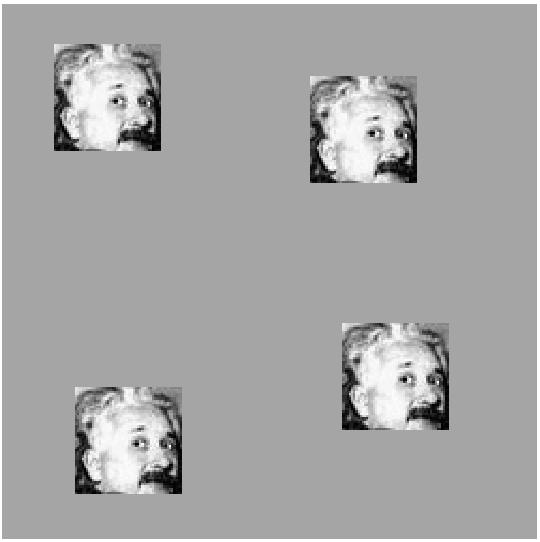
\includegraphics[scale=0.5]{micrograph_Einstein_example_clean}
		\caption{$\sigma = 0$}
	\end{subfigure}%
	\begin{subfigure}[h]{0.33\textwidth}
		\centering
		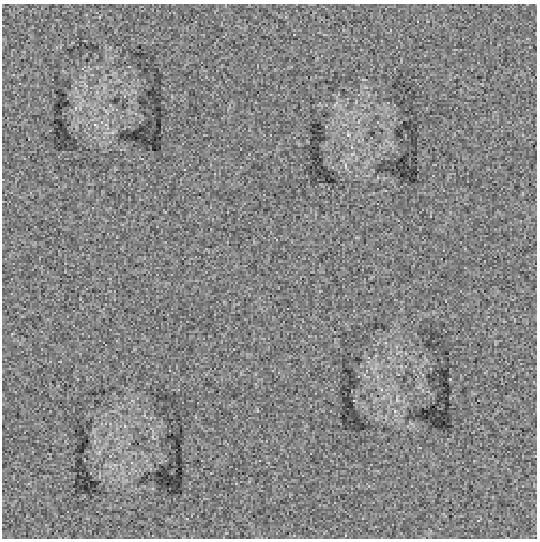
\includegraphics[scale=0.5]{micrograph_Einstein_example_s05}
		\caption{$\sigma = 0.5$}
	\end{subfigure}
	\begin{subfigure}[h]{0.33\textwidth}
		\centering
		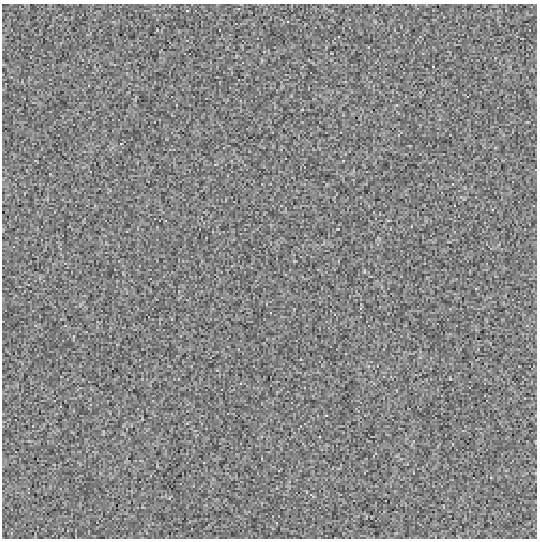
\includegraphics[scale=0.5]{micrograph_Einstein_example_s3}
		\caption{$\sigma = 3$}
	\end{subfigure}
	\caption{\label{fig:micro_example} Example of micrographs of size $250\times 250$ with additive white Gaussian noise of variance $\sigma^2$ for increasing values of $\sigma$. Each micrograph contains the same four occurrences of a $50 \times 50$ image of Einstein. In panel (c), the noise level is such that it is very challenging to locate the occurrences of the planted image. In fact, it can be shown that at low SNR, reliable detection of individual image occurrences is impossible, even if the true image is known. By analogy to cryo-EM, this depicts a scenario where particle picking cannot be done.}	
\end{figure*}


\section{Proof of concept: A mathematical toy model}

In this section, we present a toy model in order to introduce the mathematical principles enabling estimation of a signal in a low SNR regime, even when detection is impossible. Later, we discuss how these principles carry through for the SPR problem. We here formulate the model for 1-D signals to ease exposition.

Let $x\in\RL$ be the target signal and let $y\in\RN$ be the observed data, where $N \gg L$. Let  $s \in \{0, 1\}^{N-L+1}$ be a binary signal indicating (with 1's) the starting positions of all occurrences of $x$ in $y$, so that, with additive white Gaussian noise:
\begin{align}
y & =  x \ast s + \varepsilon, & \varepsilon & \sim \mathcal{N}(0,\sigma^2 I_N),
\label{eq:model}
\end{align}
where $\ast$ denotes linear convolution. 
While both $x$ and $s$ are unknown, the goal is only to estimate $x$ from $y$. The parameters of the signal $s$ (the locations of its nonzero values) are the \emph{nuisance variables} of the problem. As will be shown next, in the low SNR environment, estimating $s$ is impossible, whereas estimating $x$ is tractable under some conditions on $s$. 

We assume that the binary signals $s$ obey the following \emph{separation condition}: If $s[i] = 1$ and $s[j] = 1$  for  $i \neq j$, then $\vert i - j\vert \geq 2L-1$.
%\begin{align} 
%\textrm{If } s[i] = 1 \textrm{ and } s[j] = 1 \textrm{ for } i \neq j, \textrm{ then } |i - j| \geq 2L-1.
%\label{eq:spacing}
%\end{align}
In words: the starting positions of any two occurrences  must be separated by at least $2L-1$ positions, so that their end points are necessarily separated by at least $L-1$ signal-free entries in the micrograph.

Our problem can be interpreted as a special case of the \emph{system identification} problem. Similarly to~\eqref{eq:model}, the system identification forward model takes the form
%
\begin{math}
%
y = x\ast w + \varepsilon,  
%
\end{math} 
%
where $x$ is the unknown signal (the ``system''), $w$ is an unknown, random, input sequence, and $\varepsilon$ is an additive noise.   
The goal of this problem is to estimate $x$, usually referred to as ``identifying the system.'' The question of identifiability of $x$ under this observation model is addressed for certain Gaussian and non-Gaussian $w$ in~\cite{benveniste1980robust,kormylo1983identifiability}. In the special case where $w$, satisfying the separation condition, we obtain our model. The same observation model is used for \emph{blind deconvolution}, a longstanding problem arising in a variety of engineering and scientific applications such as astronomy, communication, image deblurring, system identification and optics; see~\cite{jefferies1993restoration,shalvi1990new,ayers1988iterative,abed1997blind}, just to name a few. 

Likelihood-based methods estimate $x$ as the maximizer of some function $f(x | y)$, where $f$ is derived from the likelihood function of $x$ given the observed signal $y$. %For example, $f$ may be the likelihood itself, or a related function with a similar form (leading to the class of ``quasi-likelihood'' methods). 
If some prior is assumed on $x$, then $f(x|y)$ can be taken to be the posterior distribution of $x$ given the data; this is the simplest form of Bayesian inference.
Methods based on such formulations are popular nowadays in cryo-EM; see for instance~\cite{sigworth1998maximum,scheres2012relion}. 
Optimizing the function $f(x|y)$ exactly is often intractable, and thus heuristic methods are used instead. One proposed technique is to use Markov Chain Monte Carlo (MCMC)~\cite{cappe1999simulation}. %Another paper considers parameterized models for multiple distinct signals, as in our framework ($K>1$)~\cite{andrieu2001bayesian}. Their proposed solution is an MCMC algorithm tailored for their specific parametrized problem. 
In special cases, including the case where $w$ is binary, expectation maximization (EM) has been used~\cite{cappe1999simulation}. The EM method for discrete $w$ is based upon a certain ``forward-backward'' procedure used in hidden Markov models~\cite{rabiner1989tutorial}. However, the complexity of this procedure is nonlinear in $N$, and therefore its usage is limited for big data sets. 
%Indeed, for a general support signal $s$, on each iteration of EM, a probability must be assigned to any feasible combination of positions for the current signal estimate in $M$ locations on the grid $\{1,\ldots,N\}$---$O(N^M)$ such combinations in total. Hence, the problem becomes computationally intractable when $M$ grows with $N$ and $N$ is large. However, exploiting the separation constraint on the support~\eqref{eq:spacing}, we devise in Section TKTK an approximate EM procedure for  our model. 
%
%Because likelihood methods are computationally expensive, methods based on recovery from moments, which are akin to our method, have also been previously used for system identification. Methods based on the third- and fourth-order moments are described and analyzed in~\cite{lii1982deconvolution,giannakis1989identification,tugnait1984identification}.

Because likelihood methods are computationally expensive, methods based on recovery from moments have also been previously used for system identification. Methods based on the third- and fourth-order moments are described and analyzed in~\cite{lii1982deconvolution,giannakis1989identification,tugnait1984identification}. Following this approach, in the next section we present an autocorrelation analysis for~\eqref{eq:model} and study it in Section~\ref{sec:theory}.  

\section{Autocorrelation analysis} \label{sec:AC_analysis}


In general, for a signal $z$ of length $m$, the autocorrelation of order $q \geq 1$ is given for any integer shifts $\ell_1, \ldots, \ell_{q-1}$ by
\begin{align}
a_z^q[\ell_1,\ldots,\ell_{k-1}]  & = \frac{1}{m} \sum_{i=-\infty}^{+\infty} z[i]z[i+\ell_1]\cdots z[i+\ell_{q-1}],
\label{eq:ac_general}
\end{align}
where indexing of $z$ out of the range $0, \ldots, m-1$ is zero-padded.
For our purposes, this will be applied both to $x$ (of length $L$) and to $y$ (of length $N$).
Explicitly, the first-, second- and third-order autocorrelations are given by \TODO{we may want to remove these explicit formulas}
\begin{align} 
a_z^1 & = \frac{1}{m} \sum_{i=0}^{m-1} z[i], \nonumber\\
a_z^2[\ell] & = \frac{1}{m} \sum_{i = \max\{0, -\ell\}}^{m-1 + \min\{0, -\ell\}} z[i]z[i+\ell], \nonumber\\
a_z^3[\ell_1,\ell_2] & = \frac{1}{m} \sum_{i = \max\{0, -\ell_1, -\ell_2\}}^{m-1 + \min\{0, -\ell_1, -\ell_2\}} z[i]z[i+\ell_1]z[i+\ell_2]. \label{eq:ac_special}
\end{align}
The autocorrelation functions have symmetries. Specifically, $a_z^2[\ell] = a_z^2[-\ell]$, and
$a_z^3[\ell_1,\ell_2] = a_z^3[\ell_2,\ell_1]=a_z^3[-\ell_1,\ell_2-\ell_1].
$

Under the spacing constraint, the relation between autocorrelations of the micrograph and those of $x$ is particularly simple. It is useful to introduce some notation: let $M$ denote the number of occurrences of $x$ in $y$ (that is, the number of 1's in $s$), and let
\begin{align}
\gamma & = \frac{M L}{N}
\end{align}
denote the density of $x$ in $y$ (that is, the fraction of entries of $y$ occupied by occurrences of $x$.) The spacing constraint%~\eqref{eq:spacing} 
imposes $\gamma\leq\frac{L}{2L-1}\approx 1/2$.

One simple observation is that the first-order\TODO{Will: I suggest making this statement about all the autocorrelations here, instead of singling out the mean first. I understand that the mean can be estimated without the separation condition, but this distinction is not very critical to highlight, and it's a little confusing to have this sentence (upon first reading, it might be interpreted to mean that the other autocorrelations do depend on s). I'd say something like: Under the separation condition on $s$, the autocorrelation functions of $y$ can be shown to depend only on the corresponding autocorrelations of $x$ and the parameter $gamma$, defined by... 
Then go into the details.} autocorrelation of $y$ (its mean) is independent of the locations of $x$. Since the noise is independent of the signal, the mathematical expectation of $a_y^1$ is easily seen to be:\TODO{Will: Instead of the footnote, just specify here that the randomness is over the Gaussian noise.
s can be deterministic. The only thing we assume about s is that the associated parameter gamma is constant (you might also note that this can be relaxed, so long as the sequence of $\gamma_N$'s converges to gamma, but this point is not critical).}\footnote{We did not fully specify a random generating model for the location vector $s$. The expectation is still well defined specifically because the quantity under consideration is independent of $s$ under the assumptions.}
\begin{align*}
\E\{ a_y^1 \} & = \gamma a_x^1.
\end{align*}
We consider the asymptotic regime where $M, N\to\infty$, while $\gamma$ remains constant (we see an increasingly large micrograph, containing increasingly many signal occurrences, with constant signal density.) In that regime, the law of large numbers can be used to show the following statement:
\begin{align} \label{eq:mean_micrograph}
\lim_{N\to\infty} a_y^1 & = \gamma a_{x}^1.
\end{align}
Thus, given enough data, if $\gamma$ is known, we can estimate $a_x^1$ from $y$. (We show later how to estimate $\gamma$ as well.)
\TODO{TB: I think that this paragraph can be much shorter and it is sufficient to show only the second equation and remove footnote. Nicolas thinks otherwise. Need to be decided. Will: I agree the footnote is unnecessary and actually confusing, since s need not be random.}

The spacing condition gives rise to more powerful observations. Consider the second-order autocorrelation in particular: $a_y^2[\ell]$ computes the correlation between $y$ and a copy of $y$ shifted by $\ell$ entries. Considering $\ell$ only in the range $0, \ldots, L-1$, one can see that any given occurrence of $x$ in $y$ is only ever correlated with itself (with the same shift $\ell$), and never with another occurrence. As a result,
\begin{align} \label{eq:ac2_micrograph}
\lim_{N\to\infty} a_y^2[\ell] & = \gamma a_{x}^2[\ell] + \sigma^2\delta[\ell]
\end{align}
for $\ell = 0, \ldots, L-1$, where $\delta$ denotes the Kronecker delta function. The last part captures the autocorrelation of the noise. Notice that, even if $\sigma$ is unknown, entries $\ell = 1, \ldots, L-1$ still provide useful information about $a_x^2$.
Along the same lines, one can establish a relation for third-order autocorrelations:
\begin{align} \label{eq:ac3_micrograph}
\lim_{N\to\infty} a_y^3[\ell_1,\ell_2] & = \gamma a_{x}^3[\ell_1,\ell_2] \\& + \sigma^2\gamma a_{x}^1 \cdot \big(\delta[\ell_1,0]+\delta[0,\ell_2]+\delta[\ell_1,\ell_2]\big), 
 \nonumber
\end{align}
for $\ell_1,\ell_2 = 0, \ldots, L-1$. Here too, few entries are affected by $\sigma$ in the limit.
Detailed derivations for identities in this and the next part are given in Appendix~\ref{sec:autocorrelation_computation}.



\section{Theory} \label{sec:theory}

If $x$ is known, then the support signal $s$ can be estimated via linear programming  in the high SNR regime~\cite{azais2015spike,denoyelle2017support,bendory2016robust,bendory2017robust}. 
However, in the low SNR regime---even if $x$ is known---estimating the binary sparse signal $s$ is impossible. 
To prove this argument, we consider an even easier problem, in which someone hands us intervals of length $L$ that either contain the full signal plus noise, or contain just noise, and we are asked to determine which intervals contain signal. 
Let us assume too that we know the signal $x$, that we know the probability $q$ that one of the intervals contains a signal, and that we know the noise variance $\sigma^2$. Since we have the full generative model, we can always generate more data as needed; therefore it is enough to consider the hardness of deciding whether a single interval contains signal or not.

Let us abstract this problem. We have two known vectors $\theta_0$ and $\theta_1$ in $\mathbb{R}^L$. There is a random variable $\eta$ taking values 0 or 1 with probabilities $q$ and $1-q$, respectively. We observe a random vector $X \in \mathbb{R}^L$ with the following distribution: $X | (\eta  = i) \sim N(\theta_i,\sigma^2)$; in other words, if $\eta = 0$, then $X \sim N(\theta_0,\sigma^2)$, and if $\varepsilon  = 1$, then $X \sim N(\theta_1,\sigma^2)$. If $\theta_1=0$, then the latter corresponds to pure noise interval.

We observe $X$, and our task is to predict $\eta$. How well can we do it? First, let us assume without loss of generality that $q \ge 1/2$. Then, if we make the constant prediction $\hat{\eta } \equiv 0$, we will be correct with probability $q$. So the question is, can we do better than this? We will prove that as $\sigma \to \infty$, the answer is no. More precisely:
\begin{proposition} \label{prop:two_gauss}
	Let $\hat{\eta }$ be any predictor of $\eta$.
	%
	\begin{align*}
	%
	\lim_{\sigma \to \infty} \P[ \hat{\eta} = \eta  ] \le q.
	%
	\end{align*}
\end{proposition}
\noindent The result is proved in Appendix~\ref{sec:proof_two_gauss}.

Proposition~\ref{prop:two_gauss} implies that in order to estimate the signal in low SNR  we must consider methods that aim to estimate the signal directly, without estimating the nuisance variables as an intermediate step. 
 %we need to consider a different approach. In this paper, we consider autocorrelation analysis.
  In what follows, we present several results on properties of autocorrelations. For simplicity, we consider one-dimensional signals, but the results carry through for higher dimensions. 

A one-dimensional signal is determined uniquely by its second- and third-order autocorrelations. Indeed, since $z[0]$ and $z[L-1]$ are nonzero by definition, we have the formula:
%
\begin{align} \label{eq-uniqueness}
%
z[k] = \frac{z[0]z[k]z[L-1]}{z[0]z[L-1]} = \frac{a_z^3[k,L-1]}{a_z^2[L-1]}.
%
\end{align}
In particular, we have proven the following proposition:
\begin{proposition} \label{prop:uniqueness}
	%
	 A signal $z\in\RL$ is determined uniquely from  $a_z^2$ and $a_z^3$.
\end{proposition}

Some remarks are in order. First, \eqref{eq-uniqueness} is not numerically stable if $z[0]$ or $z[L-1]$ are close to 0. In practice, we recover $z$ by fitting it to its autocorrelations using a nonconvex least-squares (LS) procedure, which is empirically more robust to additive noise; we have observed similar phenomena for related problems~\cite{bendory2017bispectrum,boumal2017heterogeneous,abbe2017multireference}.
Second, if the separation condition holds, then the length of the signal can be determined from the autocorrelations.
In particular, if the separation condition holds for some spacing $W\geq L$, then $a_z^2[i]=0$ for all $i>L-1$.
Third, note that the second-order autocorrelation is not by itself sufficient to determine the signal uniquely. %~\cite{beinert2015ambiguities,bendory2017fourier}.
However, for dimensions greater than one, almost all signals are determined uniquely up to sign (phase for the complex signals) and reflection through the origin (with conjugation in the complex case). %~\cite{hayes1982reconstruction,hayes1982reducible}. 
The sign ambiguity can be resolved by the mean of the signal if it is not zero. However, determining the reflection symmetry still requires additional information, beyond the second-order autocorrelation.

The observed moments $a_y^1,a_y^2$ and $a_y^3$ of $y$ do not immediately give the moments of the signal $x$, as seen by~\eqref{eq:mean_micrograph},~\eqref{eq:ac2_micrograph} and~\eqref{eq:ac3_micrograph}; rather, the two are related by the noise level $\sigma$ and the ratio $\gamma = \lim_{N\to\infty}ML/N$, \TODO{Will: Earlier, you defined gamma in the finite sample case; now it's the limit. These should be made consistent.} where $M=M_N$ grows with $N$. We will show, however, that $x$ is still identifiable from the observed moments of $y$. In general, we say a parameter is ``identifiable'' if its value is uniquely determined in the limit $N \to \infty$.

First, we observe that if the noise level $\sigma$ is known, one can estimate $\gamma$ from the first two moments of the observed vector.
%
\begin{proposition} \label{prop:gamma}
	Let $\sigma > 0$ be fixed. If the mean of $x$ is nonzero, then 
	%
	\begin{equation*}
	%
	\gamma = \lim_{N \to \infty}\frac{(a^1_y)^2}{\sum_{j=0}^{L-1}a_y^2[j]-\sigma^2} \quad \text{a.s.}
	%
	\end{equation*}
	%
\end{proposition}
\begin{proof}
	The proof follows from plugging the explicit expressions of~\eqref{eq:mean_micrograph} and~\eqref{eq:ac2_micrograph} into the right hand side of the equality.
\end{proof}

Using third-order autocorrelation information of $y$, both the ratio $\gamma$ and the noise $\sigma$ are identifiable. For the following results, when we say that a result holds for a ``generic'' signal $x$, we mean that the set of signals which cannot be determined by these measurements
lies in a set with Lebesgue measure zero. 
In particular, this means that we can recover
almost all signals with the given measurements.

\begin{proposition} \label{prop:gamma_sigma}
	%
	%Let $\sigma > 0$ be fixed. 
	The observed autocorrelations $a_y^1,a_y^2$ and  $a_y^3$ determine the ratio $\gamma$ and noise level $\sigma$ uniquely for a generic signal $x$. If $\gamma\geq\frac{L}{4(L-1)}\approx \frac{1}{4}$, then this holds for any signal $x$ with nonzero mean. 
	\begin{proof}
		See Appendix~\ref{sec:proof_prop_gamma_sigma}.
	\end{proof}
\end{proposition}

From Propositions~\ref{prop:uniqueness} and~\ref{prop:gamma_sigma} we can directly deduce the following:
\begin{corollary}
	%Let $K=1$ and $\sigma > 0$ be fixed.
	 The signal $x$, the ratio $\gamma$, and the noise level $\sigma$ are identifiable from the first three autocorrelation functions of $y$ if:
	\begin{itemize}
		\item Either the signal $x$ is generic; or
		\item   $x$ has nonzero mean  and $\gamma\geq\frac{L}{4(L-1)}$.
	\end{itemize}
\end{corollary}


\section{Numerical experiments}

The technique we advocate allows recovery of a signal hidden in noisy micrographs without (even implicitly) \TODO{Will: What does this mean?} detecting the location  of the signals embedded in these micrographs. To illustrate the underlying principles of the method, we present several numerical examples for the toy model~\eqref{eq:model} and a simple proof of concept for simulated cryo-EM data.  Appendix~\ref{sec:numeric_details} provides additional details on the experiments.

In the first experiment, we estimated 
an 50-by-50 pixel image of Einstein with mean zero from a growing number of micrographs, each of size $4096\times 4096$ pixels. Each micrograph contains, on average, 700 occurrences of the target image at random locations. 
Thus, about 10\% of each micrograph contains signal. The micrographs are contaminated with additive white Gaussian noise with standard deviation $\sigma=3$,  corresponding  to SNR = $\frac{M\|x\|_F^2} {\sigma^2N} \approx1/370$. This high noise level is illustrated in Figure~\ref{fig:micro_example}. 
To simplify the experiment, we assume the number of signal occurrences and the noise standard deviation are known. Micrographs are generated such that any two occurrences are always separated by at least 49 pixels in each direction in accordance with the separation condition. %~\eqref{eq:spacing}. %The separation restriction is discussed in more details in the Methods Section.

We compute the average second-order autocorrelation of the micrographs. This is a particularly simple computation which can be efficiently executed with a fast Fourier transform (FFT) on GPUs. Given the noise level and number of image repetitions, the second-order autocorrelation of the image can be easily deduced from~\eqref{eq:ac2_micrograph}.  Then, to estimate the target image, we resort to a standard phase retrieval algorithm called relaxed-reflect-reflect (RRR)~\cite{elser2017rrr}, initialized randomly.
Relative error is measured as the ratio of the root mean square error to the norm of the ground truth (square root of the sum of squared pixel intensities).

Figure~\ref{fig:Einst_example} shows several estimated images for a growing number of micrographs, and a movie is available in \TODO{supplementary material}. Figure~\ref{fig:error_per_micro} presents the normalized recovery error as a function of the amount of data available.  This is computed after fixing the reflection symmetries (see Section~\ref{sec:AC_analysis}). As evidenced by these figures, the ground truth image can be estimated increasingly well from increasingly many micrographs, without particle picking.
\TODO{Tamir: the experiment is currently running; should be ready tomorrow  (Aug 28).}

In practice, we do not expect to know $\gamma$ and maybe not even $\sigma$.
Figure~\ref{fig:1D_example} shows recovery of a 1-D signal from the first three autocorrelations of the data.
The autocorrelations are computed from noisy micrographs with $\sigma=3$ that obey the separation condition.% of~\eqref{eq:spacing}.
 Both the signal  and $\gamma$ are estimated simultaneously from the observed autocorrelations by LS fitting; more details are given in Appendix~\ref{sec:numeric_details}. Crucially, the LS does not require the knowledge of $\sigma$. 


\begin{figure*}[h]
	\centering
	\begin{subfigure}[h]{0.24\textwidth}
		\centering
		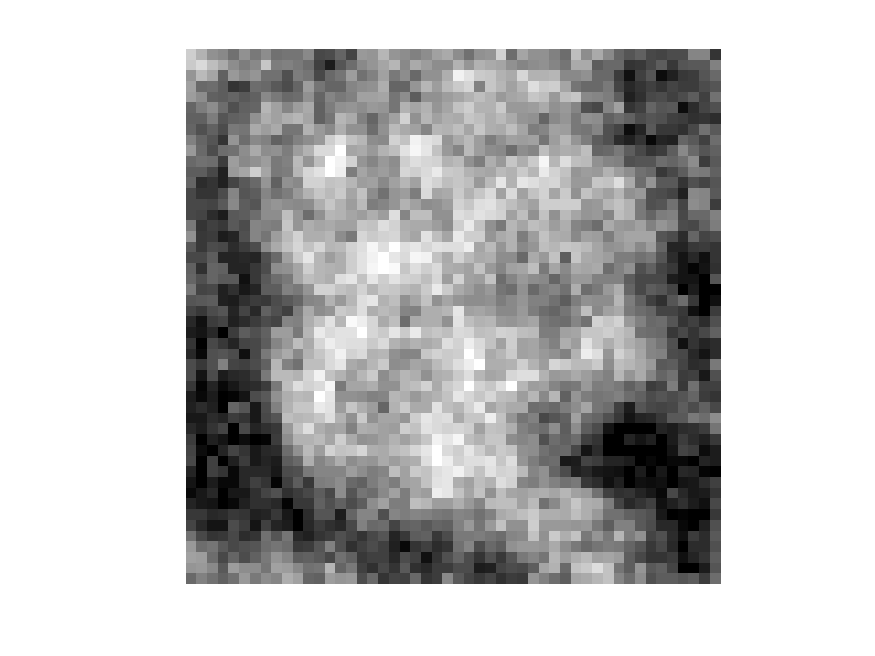
\includegraphics[scale=0.35]{Einstien_progress_1}
		\caption{$5\times 10^2$ micrographs}
	\end{subfigure} 
	\begin{subfigure}[h]{0.24\textwidth}
	\centering
	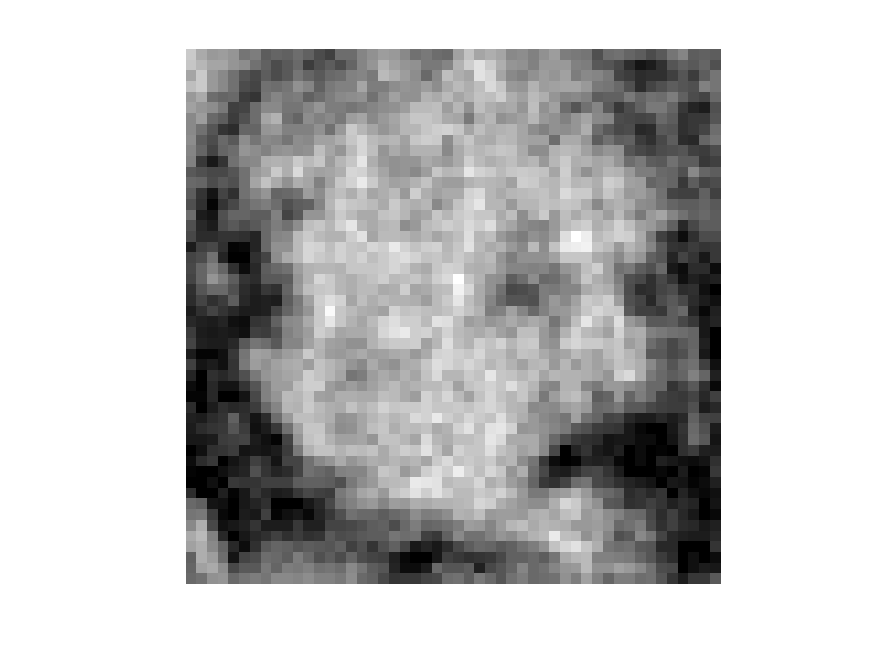
\includegraphics[scale=0.35]{Einstien_progress_10}
	\caption{$5\times 10^3$ micrographs}
\end{subfigure} 
	\begin{subfigure}[h]{0.24\textwidth}
		\centering
		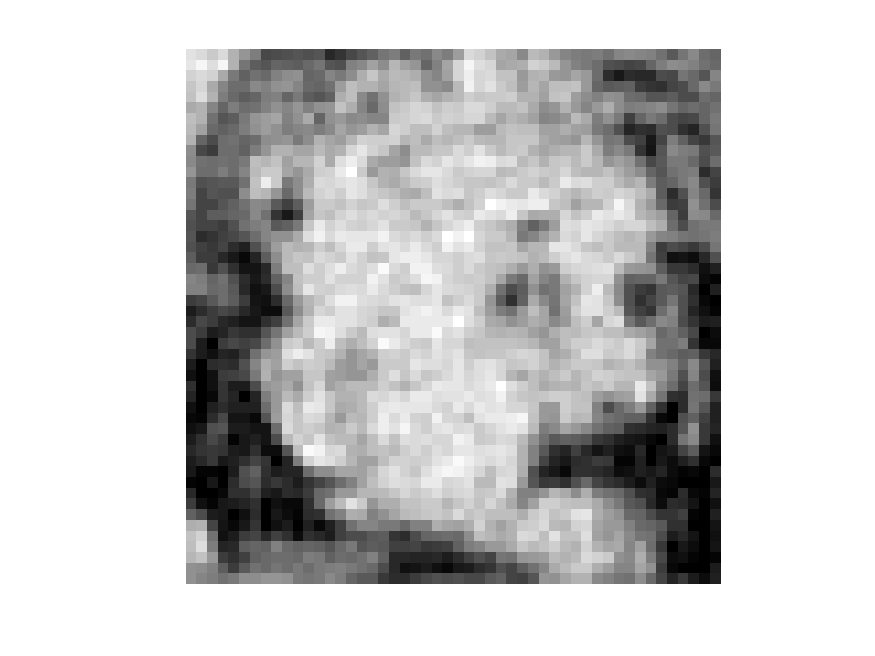
\includegraphics[scale=0.35]{Einstien_progress_100}
		\caption{$5\times 10^4$ micrographs}
	\end{subfigure} 
	\begin{subfigure}[h]{0.24\textwidth}
		\centering
		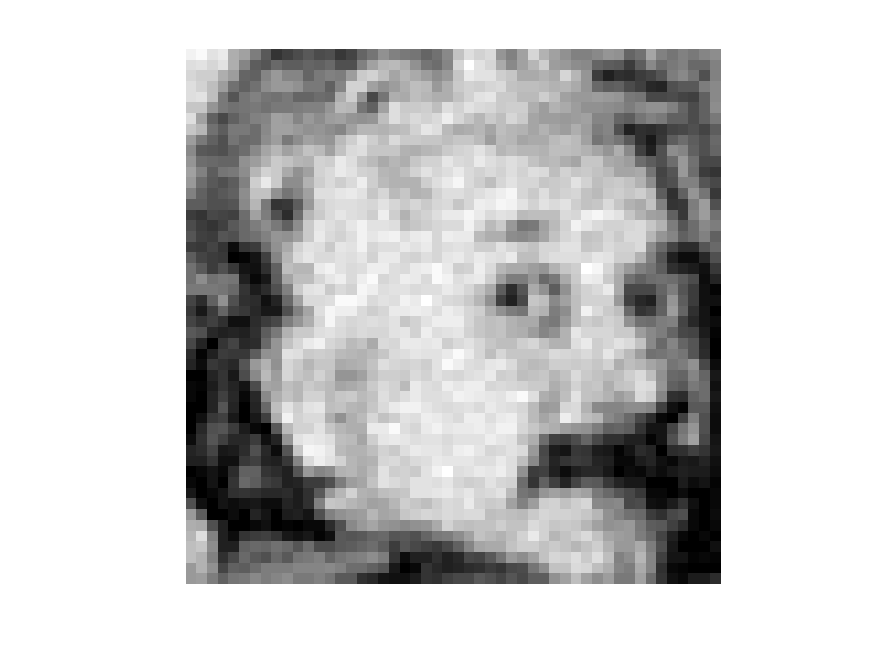
\includegraphics[scale=0.35]{Einstien_progress_246}
		\caption{$500\times 246$ micrographs}
	\end{subfigure}
	\caption{\label{fig:Einst_example} Recovery of Einstein from micrographs at noise level $\sigma = 3$ (see Figure~\ref{fig:micro_example}(c)). Averaged autocorrelations of the micrographs allow to estimate the power spectrum of the target image. This does not require particle picking. A phase retrieval algorithm (RRR) produces the estimates here shown, initialized randomly. Estimates are obtained from $5\times 10^2,5\times 10^3,5\times 10^4$ micrographs (growing across panels), each containing $700$ image occurrences on average. \TODO{XP is still running}}	
\end{figure*}


%\begin{figure*}[h!]
%	\centering
%	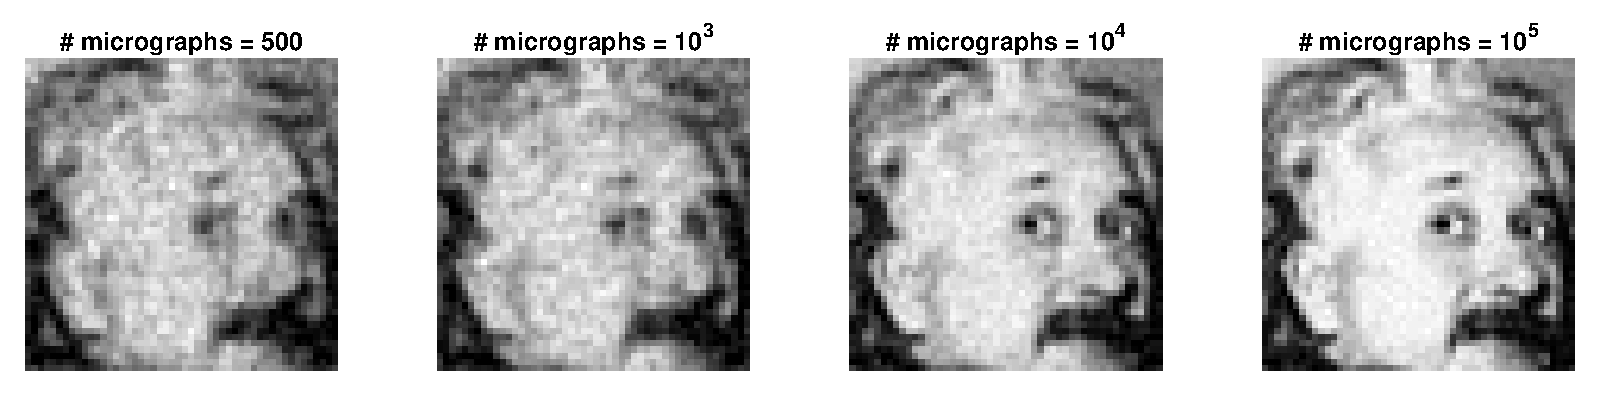
\includegraphics[scale=0.7]{Einstein_progress_examples}
%	\caption{\label{fig:Einst_example} Recovery of Einstein from micrographs at noise level $\sigma = 3$ (see Figure~\ref{fig:micro_example}(c)). Averaged autocorrelations of the micrographs allow to estimate the power spectrum of the target image. This does not require particle picking. A phase retrieval algorithm (RRR) produces the estimates here shown, initialized with an image of the physicist Isaac Newton. Estimates are obtained from $P$ micrographs (growing across panels), each containing $700$ image occurrences on average.
%		%\TODO{To add: redo the figures according to Amit's comments and the figures of noisy Einstein's micrographs}
%		% At a noise level of $\sigma = 3$, this amounts to an SNR of $1/20$.
%	}
%\end{figure*}


\begin{figure}[h]
	\centering
\begin{subfigure}[h]{0.23\textwidth}
	\centering
	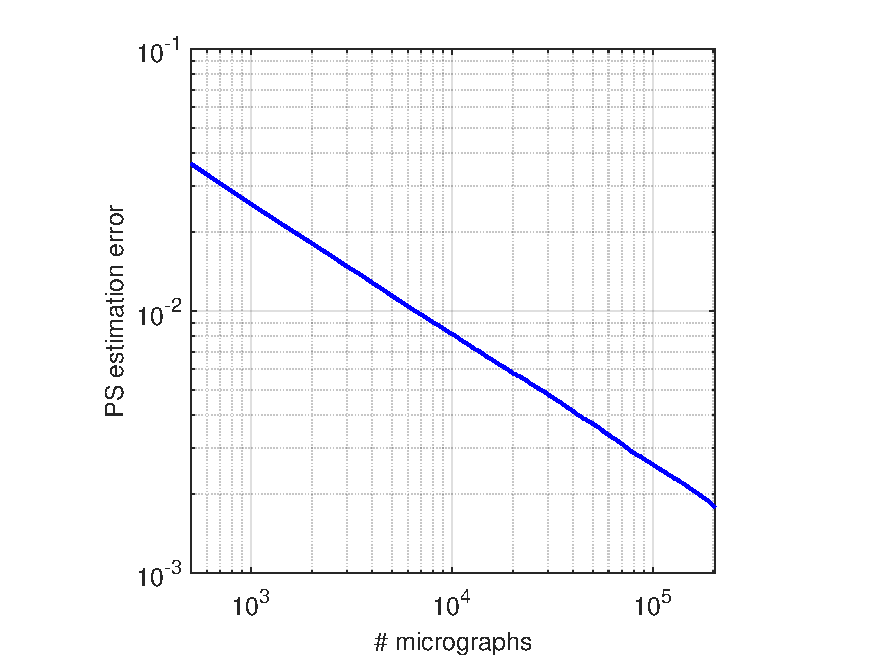
\includegraphics[scale=0.33]{Einstein_ps_error}
	\caption{relative power spectrum estimation error}
\end{subfigure} 
\begin{subfigure}[h]{0.23\textwidth}
	\centering
	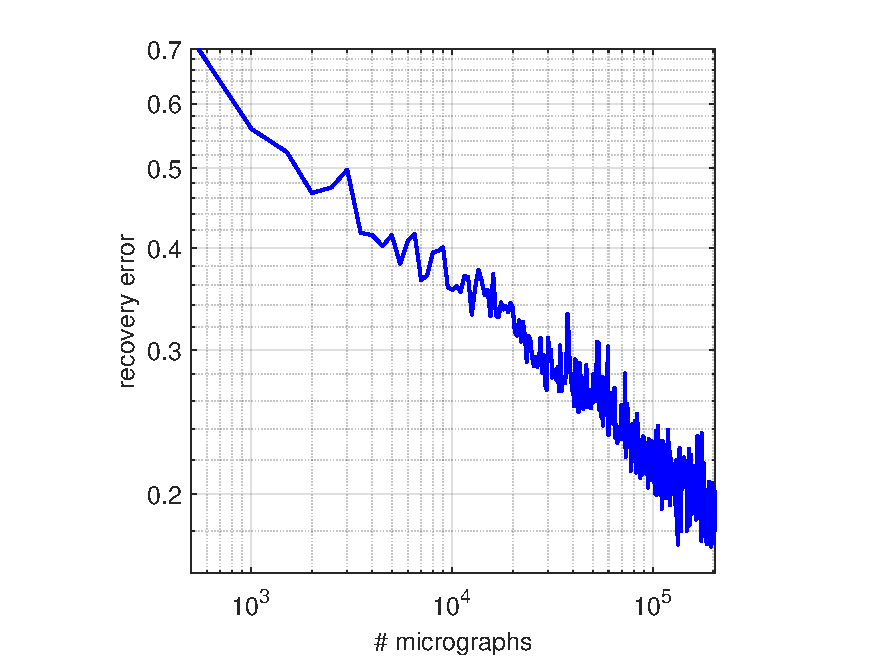
\includegraphics[scale=0.33]{Einstein_recovery_error}
	\caption{relative recovery error}
\end{subfigure} 
	\caption{\label{fig:error_per_micro} Error curves for the experiment of Figure~\ref{fig:Einst_example} \TODO{XP is still running}}
\end{figure}

%
%\begin{figure}[h]
%	\centering
%	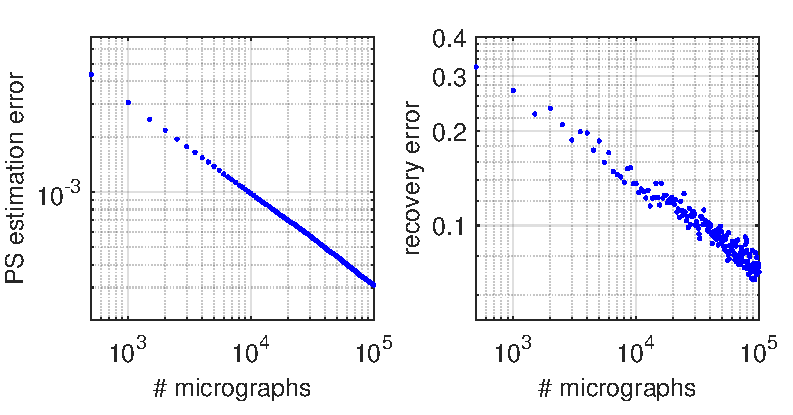
\includegraphics[scale=.55]{Einstein_progress} (left) power spectrum estimation error (right) RRR error after fixed number of 1000 iterations.
%	\caption{\label{fig:error_per_micro} Relative root mean square error of the estimate of Einstein's image as a function of the number of observed micrographs (logarithmic scale along both axes.)}
%\end{figure}



\begin{figure*}[h!]
	\centering
	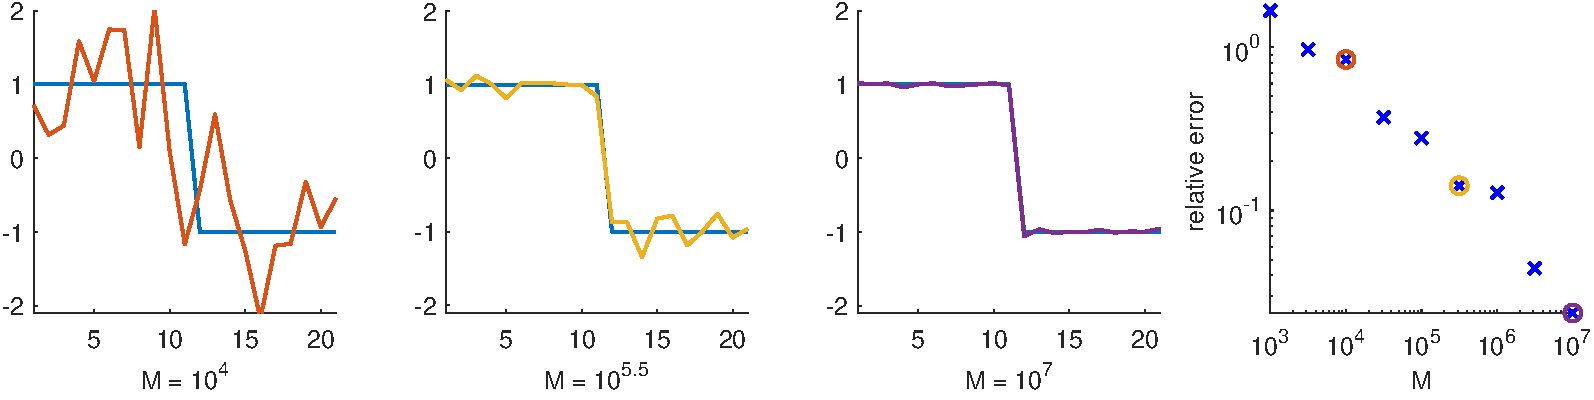
\includegraphics[scale=0.7]{1D_example}
	\caption{\label{fig:1D_example} Recovery of a 1-D signal of length $L=21$ at noise level $\sigma = 3$ from $M$ repetitions. The length of the micrograph was set to be $N = 410*M$. The first three panels (left to right) show reconstruction with different $M$ values compared to the ground truth signal (in blue).
		The true value of $\gamma$ is $0.0512$.
		   The relative errors of $\gamma$ for the three panels are: $27.1\%,4\%,1.2\%$. The right panel shows the relative error as a function of $M$.
	}
\end{figure*}

The application of autocorrelation analysis to cryo-EM follows the same mathematical principles.
The derivation of the first three autocorrelations of the micrographs and their relations to the volume itself are provided in Appendix~\ref{sec:ac_cryo}.
In particular, numerical evidence suggests that the third-order autocorrelation uniquely determines the 3-D volume. Figure~TKTK shows recovery of the 3-D volume from the clean autocorrelations. The details of the reconstruction algorithm are given in Appendix~\ref{sec:numeric_details}.
Unfortunately, the mapping between the autocorrelations and volume seems to be ill-conditioned, preventing recovery from noisy data. 
In the next section, we outline how we suggest to overcome the ill-conditioning in future work. 

While we cannot provide a 3-D reconstruction from noisy data with the current algorithm, our method can be easily applied to the problem of deciding whether a micrograph contains projections or merely pure noise---a problem considered in classical works in statistics (e.g.,~\cite{donoho2004higher}) and debates in the cryo-EM community~\cite{henderson2013avoiding}.
This task can be performed by considering solely the recovered $\gamma$ (the fraction of pixels occupied by projections in the micrograph), estimated as part of the recovery algorithm.
Figure~\ref{fig:cryo_detection} presents excerpts \TODO{sections?} of two noisy micrographs, only one of which contains projections.
In the presence of projections, the estimated $\gamma$ was $0.12$, corresponding to approximately $6784$ projections. 
On the hand, the estimated $\gamma$ drops to $10^{-5}$ for the pure noise micrograph, corresponding to less than one projection.
%
%Under the experimental parameters (see Section~\ref{sec:numeric_details}), such values of $\gamma$ predict  in the informative micrograph and less than one projection in the pure noise scenario.  

\begin{figure*}[h]
	\centering
	\begin{subfigure}[h]{0.3\textwidth}
		\centering
		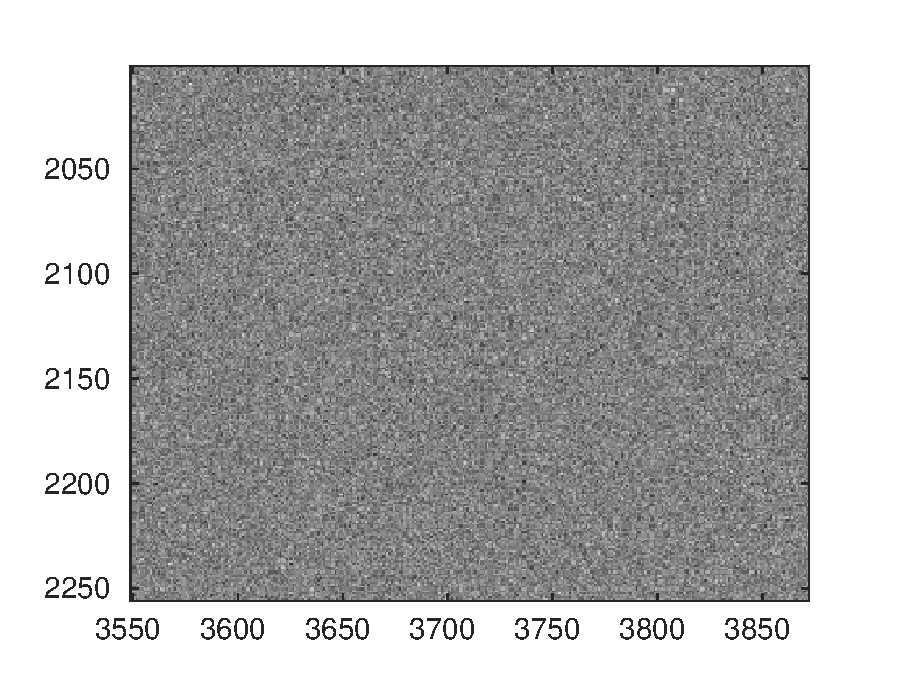
\includegraphics[scale=0.4]{pure_noise_micrograph_cutout.eps}
		\caption{An excerpt of the pure noise micrograph}
	\end{subfigure} \hspace{2pt}
	\begin{subfigure}[h]{0.3\textwidth}
		\centering
		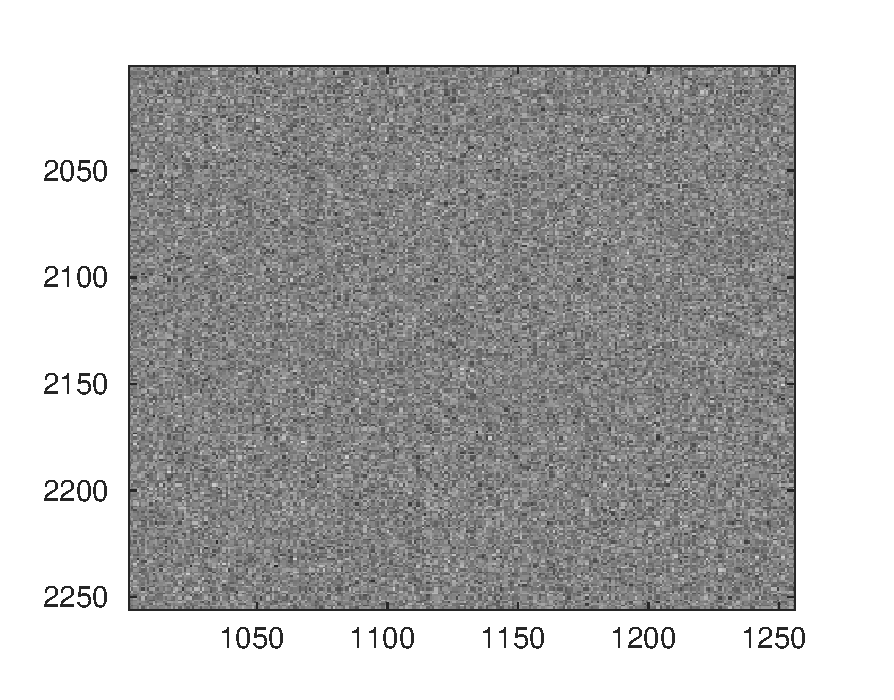
\includegraphics[scale=0.4]{noisy_micrograph_cutout.eps}
		\caption{An excerpt of the clean micrograph in right panel perturbed by the noise in the left panel.}
	\end{subfigure} \hspace{2pt}
	\begin{subfigure}[h]{0.3\textwidth}
		\centering
		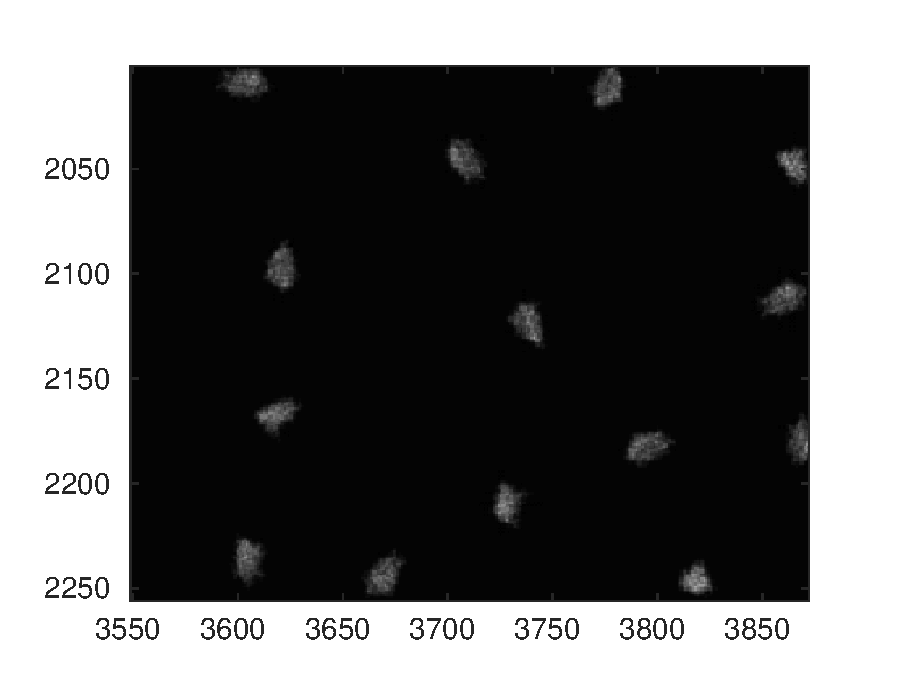
\includegraphics[scale=0.4]{clean_micrograph_cutout.eps}
		\caption{An excerpt of the clean micrograph}
	\end{subfigure}
	\caption{\label{fig:cryo_detection} All micrographs are of size $7420^2$ pixels and the projections are taken from a volume of size $31^3$. The added noise was drawn from i.i.d.\ Gaussian distribution with zero mean and standard deviation $25$, corresponding to an SNR below $1/1024$.  
		The noise realization is identical in both micrographs. }	
\end{figure*}



\section{Discussion}

%In the simplified model for cryo-EM we examined, we showed it is possible to estimate the 3-D structure of small volumes. 
In the simplified mathematical model we examined, we showed it is possible to estimate a signal without detecting its appearances.  
Our strategy is to compute autocorrelation functions of the micrographs and to relate these statistics to the unknown signal's parameters. Recovering the parameters from the statistics reduces to solving a set of polynomial equations. 

We also showed how this technique can, in principle, be applied to cryo-EM.
Crucially, the outlined approach involves no particle picking, hence a fortiori no viewing direction estimation. Concerns for model bias are also greatly reduced since no template matching is involved.
Additionally,  our technique also allows the use of much lower defocus values. Lower defocus means lower contrast, but will maintain  higher frequency information. Consequently, we may be able to get high resolution reconstructions from fewer micrographs.


Looking towards applying the framework to encompass all important features of real cryo-EM experiments, our work implies that it might be possible to reconstruct small molecules, particularly, molecules that are too small to be detected in micrographs. 
In pursuing this research direction, our goal is to significantly increase the range of molecules to which cryo-EM can be successfully applied.
We recognize that significant challenges lay ahead for the implementation of the proposed approach to 3-D reconstruction directly from the micrographs. We discuss a few now.

\TODO{First and foremost, we need to mention the sensitivity of the third moment and whether the fourth moment is enough}
%As a result, it may not be limited to large molecules in the same way that particle picking approaches are. 
%In this paper, we illustrated that it is possible to determine the 3-D molecular structure in single particle cryo-EM directly from the micrographs without performing particle picking, at least in controlled experiments. 

%
%\TODO{
%	We should also incorporate Alberto's comment that our technique also allows to use much lower defocus values. Lower defocus means lower contrast, but will maintain higher frequency information. From that perspective, we may be able to get high resolution reconstructions from fewer micrographs, just because we would be using lower defocus. }

%All current algorithmic pipelines for SPR using cryo--EM start with a particle picking algorithm which is prone to model bias. 
%Bypassing the particle picking stage and constructing a 3-D model directly from the data---without assuming prior knowledge on the particle to be estimated---can be used to reconstruct ab initio models to initialize a refinement algorithm.  Alternatively, it can be applied to generate templates for a particle picker which does not suffer from model bias.


%In the simplified model we examined, the aim is to estimate one, or possibly several, images from micrographs. Our strategy is to compute autocorrelation functions of the data and to relate these statistics to the unknown parameters. Recovering the parameters from the statistics reduces to solving a set of polynomial equations. Depending on the scenario, we did so using either a phase retrieval algorithm or a nonlinear least-squares algorithm.
%


%Depending on the scenario, we did so using either a phase retrieval algorithm or a nonlinear least-squares algorithm.

%
%The same general approach can, in principle, be applied directly to SPR from cryo-EM. Here, the micrographs contain numerous tomographic projections of molecules (possibly in different conformations) taken from unknown viewing directions. The aim is to estimate the 3-D volumes of the different conformations directly from micrographs. Each volume can be expanded linearly in a basis, so that the volume is characterized by its expansion coefficients. Since tomographic projection is a linear operation, autocorrelations of the micrographs (which can be estimated easily) are polynomial functions of the sought coefficients. Thus, autocorrelations of the micrographs provide a system of polynomial equations in the volume parameters, and the question becomes: are these equations sufficient to uniquely identify the volumes, and can we solve the system?
%
%We show in Appendix~\ref{sec:cryoem} that the number of polynomial equations provided by the third-order autocorrelations is of the same order as the number of coefficients required to describe one volume \TODO{at resolution comparable to that of the particle projections---remove?}. This hints that it may be possible to reconstruct one or even several distinct volumes from these equations directly. Additional parameters in these equations could encode an unknown viewing direction distribution and an unknown conformation distribution, which could then also be estimated. Crucially, the outlined approach involves no particle picking, hence a fortiori no viewing direction estimation or conformation clustering. As a result, it may not be limited to large molecules in the same way that particle picking approaches are. Concerns for model bias would also greatly be reduced.


%While the field is currently dominated by Bayesian methods such as EM, they are intractable for such problems. As an alternative, we propose to use autocorrelation analysis technique that shares some common lines (did you get the wordplay?)  with Kam's method for ab initio modeling~\cite{kam1980reconstruction,levin20173d,singer2018mathematics}. That being said, the SPR model is far more complicated than the model presented here. In a future research, we hope to bridge this gap.

One possible concern is that the numerical experiments conducted here suggest a large amount of data may be necessary.\footnote{Whether or not this large amount of data would be necessary for any method to succeed given the unfavorable SNR remains an open question.} Recent trends in high-throughput cryo-EM technology \TODO{?} give hope that this may be a lesser concern in the long term. Still, large amounts of data also require large amounts of computation. On this front, we note that computing autocorrelations can be executed efficiently on CPUs and GPUs, and in parallel across micrographs. It can even be done in streaming mode, as only one pass through each micrograph is necessary. The output of this data processing stage is a succinct summary in the form of autocorrelation estimates: its size is a function of the resolution, not a function of the number of observed micrographs. Subsequent steps, which involve solving the system of polynomial equations, scale only in the size of that summary. Of course, an important question then is whether the equations can be solved meaningfully in practice. The proof-of-concept experiments above suggest they might. \TODO{Is it?}

Beyond data acquisition and computational challenges, there are modeling issues to consider.
As stated, our approach relies on two core assumptions that are not necessarily verified in SPR experiments.
First, we assume an additive white noise model, while in practice the noise may be correlated or signal dependent. To address this point, it may be necessary to investigate better noise models and to incorporate power spectrum estimation methods. % and to extend the autocorrelation analysis accordingly. 
Second, we assume that any two particles are sufficiently separated, and we use this assumption to derive algebraic relations between autocorrelations of the micrographs and autocorrelations of the 3-D volume. 
We believe that this constraint could be replaced by a probabilistic condition on the average number of projections per micrograph.\TODO{Will: Is this really enough? I think the main issue is what happens when particles can collide (or maybe even overlap), since this introduces additional cross-terms for the moment-fitting problem.} 
Such a condition can be met in practice by careful experimental design.

We also note several aspects of SPR experiments that were neglected in this paper, including contrast transfer function (CTF), non-uniformity of the viewing directions \TODO{We never talk about viewing directions at all, so it's strange to mention that non-uniformity is an issue. I think this is confusing. I'd say something like: "relating the observed autocorrelations to the autocorrelations of the 3-D volume" or something like that.} and other contaminants in the micrographs, such as ice crystals.
 All these aspects must be taken into account so the method could be applied on real data. We hope to take care of these issues in future research, as well to extend the proposed method to conformational heterogeneity. 

% Bibliography
\bibliography{ref}


\appendix

\section{Numerical experiments details} \label{sec:numeric_details}

\paragraph{2-D experiment.}

For the 2-D experiment shown in Figures~\ref{fig:Einst_example} and~\ref{fig:error_per_micro}, we generate $P$ micrographs of size $4096\times 4096$ pixels. 
In each micrograph, we place Einstein's image (of zero mean) of size $50\times 50$  in random locations, while preserving the separation condition.%~\eqref{eq:spacing}.  
This is done by randomly selecting $4000$ placements in the micrograph, one at a time with
an accept/reject rule based on the separation constraint and locations picked so far.
On average, $700$ images are placed in each micrograph.   
Then, i.i.d.\ Gaussian noise with standard deviation $\sigma=3$ is added, inducing an SNR of approximately $1/375$.
An example of a micrograph's excerpt is presented in the right panel of Figure~\ref{fig:micro_example}.
%Different micrographs are handled sequentially on a GPU, as GPUs are particularly well suited to execute simple instructions across large vectors of data. If multiple GPUs are available, segments can of course be handled in parallel.


In this experiment, we assume we know the noise level $\sigma$ and the total number of occurrences of the target image across all micrographs.
In stark contrast with the 1-D setup, the second-order autocorrelation determines almost any target image uniquely, up to reflection through the origin. This is because the second-order autocorrelations correspond to the Fourier magnitudes of the signal through the 2-D Fourier transform. 
Therefore, we estimate the signal's Fourier magnitudes (or power spectrum) from the Fourier magnitudes of the micrographs, at the cost of one 2-D fast Fourier transform (FFT) per micrograph. These can be computed highly efficiently and in parallel.

To recover the target image from the estimated power spectrum, we use a standard phase retrieval algorithm called relaxed-reflect-reflect (RRR). This algorithm iterates the map
\begin{align*}
z & \leftarrow z + \beta (P_2(2P_1(z) - z) - P_1(z))
\end{align*}
on an image $z$ of size $2L\times 2L$.
We set the parameter $\beta$ to 1.
The map is designed so that, if the estimated power spectrum is exact, then fixed points contain Einstein's image in the upper-left corner of size $L \times L$, possibly reflected through its origin, and zeros elsewhere. The operator $P_2(z)$ combines the Fourier phases of  the current estimation $z$ with the estimated Fourier magnitudes. The operator $P_1(z)$ zeros out all entries of $z$ outside the $L\times L$ upper-left corner. In all experiments, the algorithm halted after a fixed number of 2000 iterations.
%
%In order to compare the performance in multiple cases and at different noise levels,  and the iterate with the smallest error compared to the ground truth (up to the reflection ambiguity) is chosen as the solution. While this cannot be done in practice (since we do not have access to the ground truth to determine which iterate is best), this procedure enables us to compare a large number of instances in different noise environments. \TODO{Note the last two sentences!}




\paragraph{1-D experiment.}
For the 1-D experiment depicted in Figure~\ref{fig:1D_example}, we used a signal of length $L=21$ and generated an observation $y$ of length $N = 10(2L-1)M$, where $M$ is the number of repetitions. 
The observation was generated by randomly selecting placements in $y$, one at a time with an accept/reject rule based on the separation constraint and locations picked so far until reaching the desired number of signal occurrences. Then, i.i.d.\ Gaussian noise with mean zero and standard deviation $\sigma = 3$ is added, to form the observed $y$. The resulting SNR of $y$ is about $1/175$.
%	 fix $K = 3$ signals of length $L = 21$. Following the forward model described at the beginning of this section, we generate an observation $y$ of length $12.3 \cdot 10^9$. Each of the three signals appears, respectively (and approximately), $30.0 \cdot 10^6$, $20.0 \cdot 10^6$ and $10.0 \cdot 10^6$ times in $y$ for a total of exactly $60 \cdot 10^6$ occurrences, such that at least $L-1$ zeros separate any two occurrences of any signals. 
%This is done by randomly selecting $60 \cdot 10^6$ placements in $y$, one at a time with an accept/reject rule based on the separation constraint and locations picked so far. For each placement, one of the three signals is picked at random according to the proportions $1/2, 1/3, 1/6$. Then, i.i.d.\ Gaussian noise with mean zero and standard deviation $\sigma = 3$ is added, to form the observed $y$. The resulting SNR of $y$
%% sqrt((m_want*sum(X.^2)')/(sigma^2*n))
%is about 1/9.


%This is enough noise to make cross-correlations of $y$ even with the true signals display peaks at essentially random locations, uninformative of the actual locations of the signal occurrences. Thus, we contend that it would be difficult for any algorithm to locate the signal occurrences, let alone to classify them according to which signal appears where.

%\TODO{TB: I would place the equation counting argument in the theory section in the paragraph of open questions (I marked th place)}
%
Given the observation $y$, we proceed to compute the autocorrelations. %The first-order autocorrelation is straightforward. 
We excluded biased elements of the autocorrelations; that is $a_y^2[\ell_1]$ and $a_y^3[\ell_1, \ell_2]$ such that $\ell_1, \ell_2$ or $\ell_1 - \ell_2$ are zero. 
This has the  practical effect that we need not know $\sigma$. 
%For second-order autocorrelations, notice from equation~\eqref{eq:data_ac} that $a_y^2[\ell]$ suffers no noise-induced bias for $\ell$ in $1$ to $L-1$. Thus, we omit $\ell = 0$, which has the practical effect that we need not know $\sigma$ to make sense of the computed quantities. Likewise, for third-order autocorrelations, $a_y^3[\ell_1, \ell_2]$ for $0 \leq \ell_1, \ell_2 \leq L-1$ such that $\ell_2 \leq \ell_1$ includes all relevant entries for our purpose (this accounts for symmetries), and we further exclude any such that $\ell_1, \ell_2$ or $\ell_1 - \ell_2$ are zero to avoid the need to estimate $\sigma$---
By also taking symmetries into account, the third-order autocorrelation contains $\frac{(L-1)(L-2)}{2}$ remaining entries. Thus, in total we have
\begin{align*}
1 + (L-1) + \frac{(L-1)(L-2)}{2} = \frac{1}{2} L (L-1) + 1
\end{align*}
coefficients. 
This redundancy suggests that it might be possible to estimate several signals simultaneously (compare with~\cite{boumal2017heterogeneous,bandeira2017estimation}).
%Since we aim to estimate $KL$ parameters (for the $K$ signals of length $L$) plus $K$ parameters (for the densities $\gamma_k$), an absolute upper bound on $K$ (simply to ensure we have at least as many equations as we have unknowns) is
%\begin{align*}
%K(L+1) \leq \frac{1}{2} L (L-1) + 1.
%\end{align*}
%Thus, $(L-1)/2$ (up to a small approximation) is an absolute upper limit on $K$ (compare with~\cite{boumal2017heterogeneous,bandeira2017estimation}). 
In practice, the autocorrelations are computed on disjoint segments of $y$ of length $100\cdot10^6$ (if the length of the measurement is larger than that) and added up, without correction for the junction points. Segments are handled sequentially on a GPU, as GPUs are particularly well suited to execute simple instructions across large vectors of data. If multiple GPUs are available, segments can of course be handled in parallel.

%Having computed the moments of interest, we now estimate signals $x_1, \ldots, x_K$ and coefficients $\gamma_1, \ldots, \gamma_K$ which agree with the data. We choose to do so by running an optimization algorithm on the following nonlinear least-squares problem:
Having computed the moments of interest, we now estimate the signal $x$ and coefficient $\gamma$ which agree with the data. We choose to do so by running an optimization algorithm on the following nonlinear LS problem:
%\begin{align}
%\min_{\substack{\hat x_1, \ldots, \hat x_K \in \mathbb{R}^{W} \\ \hat \gamma_1, \ldots, \hat \gamma_K > 0}}& w_1 \left( a_y^1 - \sum_{k=1}^K \hat \gamma_k a_{\hat x_k}^1 \right)^2 \\ & + w_2 \sum_{\ell = 1}^{L-1} \left( a_y^2[\ell] - \sum_{k=1}^K \hat \gamma_k a_{\hat x_k}^2[\ell] \right)^2  \nonumber \\&+ w_3 \sum_{\substack{2\leq\ell_1\leq L-1 \\ 1 \leq \ell_2 \leq \ell_1-1}} \left( a_y^3[\ell_1, \ell_2] - \sum_{k=1}^K \hat \gamma_k a_{\hat x_k}^3[\ell_1,\ell_2] \right)^2, \nonumber
%\label{eq:optim1D}
%\end{align}
\begin{align}
\min_{\substack{\hat x\in \mathbb{R}^{W} \\ \hat \gamma > 0}}& w_1 \left( a_y^1 - \hat \gamma a_{\hat x}^1 \right)^2  + w_2 \sum_{\ell = 1}^{L-1} \left( a_y^2[\ell] - \hat \gamma a_{\hat x}^2[\ell] \right)^2  \nonumber \\&+ w_3 \sum_{\substack{2\leq\ell_1\leq L-1 \\ 1 \leq \ell_2 \leq \ell_1-1}} \left( a_y^3[\ell_1, \ell_2] -  \hat \gamma a_{\hat x}^3[\ell_1,\ell_2] \right)^2, 
\label{eq:optim1D}
\end{align}
where $W \geq L$ is the length of the sought signals and the weights are set to $w_1 = 1/2, w_2 = 1/2n_2, w_3 = 1/2n_3$, where $n_2, n_3$ are the number of moments used: $n_2 = L-1$, $n_3 = \frac{(L-1)(L-2)}{2}$ (weights could also be set in accordance with variance estimates as in~\cite{boumal2017heterogeneous}).

Setting $W = L$ (as is a priori desired) is problematic because the above optimization problems appears to have numerous poor local optimizers. Similar phenomenon was recently observed in a related problem~\cite{zhang2018structured}.
Thus, we first run the optimization with $W = 2L-1$. This problem appears to have few poor local optima, perhaps because the additional degrees of freedom allow for more escape directions. Since we hope the signals estimated this way correspond to the true signals zero-padded to length $W$, we extract from each one a subsignal of length $L$ that has largest $\ell_2$-norm. This estimator is then used as initial iterate for~\eqref{eq:optim1D}, this time with $W = L$. We find that this procedure is reliable for a wide range of experimental parameters. To solve~\eqref{eq:optim1D}, we run the trust-region method implemented in Manopt~\cite{manopt}, which allows to treat the positivity constraints on coefficients $\hat \gamma$. Notice that the cost function is a polynomial in the variables, so that it is straightforward to compute it and its derivatives.

\paragraph{3-D experiments.}

For the experiment in Figure~TKTK, we computed the analytical first three autocorrelations of the volume according to~TKTK. To estimate the coefficients of the volume itself, we solve the LS problem
\begin{equation} \label{eq:LS_cryo}
\min_{\hat{x},\hat{\gamma}} w_1 \vert \mathfrak{a}_x^1 - \hat{\gamma}\mathfrak{a}_{\hat{x}}^1 \vert^2 + w_2\| \mathfrak{a}_x^2 - \hat{\gamma}\mathfrak{a}_{\hat{x}}^2 \|_2^2 + w_3\| \mathfrak{a}_x^3 - \hat{\gamma}\mathfrak{a}_{\hat{x}}^3 \|_F^2, 
\end{equation}  
where the explicit expressions of $\mathfrak{a}_x^1$, $\mathfrak{a}_x^2$ and $\mathfrak{a}_x^3$ are given in~\eqref{eq:ac_1_prolates},~\eqref{eq:ac_2_prolates} and~\eqref{eq:ac_3_prolates}, respectively.  
In the experiments, we set $w_1=w_2=w_3=1$. 

The LS was solved by TKTK. The expected $\hat \gamma$ is one.

In the first experiment, we used \TODO{Bla bla bla, real valued volume}

The micrographs for the experiment presented in Figure~\ref{fig:cryo_detection} were generated as follows \TODO{separation, etc. }. Then, the LS~\eqref{eq:LS_cryo} was solved with $L=0$ (low-resolution estimate).

\section{Derivation of the identities in Section~\ref{sec:AC_analysis}} \label{sec:autocorrelation_computation}

Throughout the proof, we consider the case of one signal $K=1$. The extension to $K>1$ is straightforward by averaging the contributions of all signal with  appropriate weights; see~\cite{boumal2017heterogeneous}. 

We will let the number of instances of the signal $M$ grow with $N$, and write $M=M_N$ to emphasize this. We assume $M_N$ grows proportionally with $N$, and define:
%
\begin{equation}
\gamma = \lim_{N\to\infty} \frac{M_NL}{N}<1.
\end{equation}
%
We will assume that $M_N=\Omega(N)$, so that $\gamma>0$. In the sequel, we will suppress the explicit dependence of $M$ on $N$ for notational convenience.

We start by considering the mean of the data:
%
\begin{equation}
a_y^1 = \frac{1}{N}\sum_{i=0}^{N-1} y[i] =
\frac{1}{N/L}\sum_{j=0}^{M-1}\frac{1}{L}\sum_{i=0}^{L-1}x[i] +    
\underbrace{\frac{1}{N}\sum_{i=0}^{N-1}\varepsilon[i]}_{\text{noise term}}
\xrightarrow{a.s.}\gamma a_x^1,
\end{equation}
%
where the noise term converges to zero almost surely (a.s.) by the strong law of large numbers.

We proceed with the (second-order) autocorrelation for fixed $\ell\in[0,\ldots,L-1]$. We can compute:
%
\begin{align*}
%
a_y^2[\ell] & = \frac{1}{N}\sum_{i=0}^{N-1-\ell}y[i]y[i+\ell]
\nonumber \\
& = \underbrace{\frac{1}{N}\sum_{j=1}^{M}\sum_{i=0}^{L-\ell-1}x[i]x[i+\ell]}_{\text{signal term}} + \underbrace{\frac{1}{N}\sum_{i=0}^{N-1-\ell}\varepsilon[i]\varepsilon[i+\ell]}_{\text{noise term}}
\\ & + \underbrace{\frac{\TODO{1,2?}}{N} \sum_{j=1}^{M} \sum_{i=0}^{L-1} x[i] \varepsilon[s_j + i + \ell]}_{\text{cross-term}}. 
%
\end{align*}

The cross-terms are linear in the noise, and are easily shown to vanish almost surely in the limit $N\to\infty$, by the strong law of large numbers. As for the signal term, we break it into $M$ different sums, each containing one copy of the signal. This gives:
%
\begin{equation} \label{eq:2nd_moment_signal_term}
%
\frac{1}{N}\sum_{j=1}^{M}\sum_{i=0}^{L-\ell-1}x[i]x[i+\ell] = \frac{ML}{N}\frac{1}{L}\sum_{i=0}^{L-\ell-1}x[i]x[i+\ell]\xrightarrow{N\to\infty}\gamma a_x^2[\ell].
%
\end{equation}
%

We next analyze the pure noise term. When $\ell\neq 0$, we can break the noise term into a sum of independent terms:
%
\begin{equation}
%
\frac{1}{N}\sum_{i=0}^{N-1-\ell} \varepsilon[i]\varepsilon[i+\ell] = \frac{1}{\ell}\sum_{i=0}^{\ell-1}\frac{1}{N/\ell}\sum_{j=0}^{N/\ell -1} \varepsilon[j\ell + i] \varepsilon[(j+1)\ell + i].
%
\end{equation}
%
Each sum $\frac{1}{N/\ell}\sum_{j=0}^{N/\ell -1} \varepsilon[j\ell + i] \varepsilon[(j+1)\ell + i]$ is an average of $N/\ell$ independent terms with expectation zero, and thus converges to zero almost surely as $N\to\infty$. If $\ell=0$, then we have:
%
\begin{equation}
%
\frac{1}{N}\sum_{i=0}^{N-1} \varepsilon^2[i] \xrightarrow{a.s.} \sigma^2.
%
\end{equation}

We now analyze the third-order autocorrelation. Let us fix $\ell_1\geq\ell_2\ge0$. We have:
%
\begin{align}
%
&a_y^3[\ell_1,\ell_2] 
= \frac{1}{N}\sum_{i=0}^{N-1-\ell_1} y[i]y[i+\ell_1]y[i+\ell_2]
\nonumber \\
%
=& \underbrace{ \frac{ML}{N}\frac{1}{M}\sum_{j=1}^M 
	\frac{1}{L}\sum_{i=0}^{L-1-\ell_1}x[i]x[i+\ell_1]x[i+\ell_2]   }_{(1)}
\\& + \underbrace{\frac{1}{N}\sum_{i=0}^{N-1-\ell_1} \ep[i]\ep[i+\ell_1]\ep[i+\ell_2]}_{(2)}
\nonumber \\
&+ \underbrace{\frac{1}{N}\sum_{j=1}^{M} 
	\sum_{i=0}^{L-1} x[i]\ep[s_j + i+\ell_1]\ep[s_j+ i+\ell_2]}_{(3)}
\\& + \underbrace{\frac{1}{N}\sum_{j=1}^{M} 
	\sum_{i=0}^{L-1} \ep[s_j+i-\ell_1]x[i]\ep[s_j+ i+\ell_2-\ell_1]}_{(4)}
\nonumber \\
&+ \underbrace{\frac{1}{N}\sum_{j=1}^{M} 
	\sum_{i=0}^{L-1} \ep[s_j+i-\ell_2]\ep[s_j+i+\ell_1-\ell_2]x[i]}_{(5)}
\\ & + \underbrace{\frac{1}{N}\sum_{j=1}^{M} 
	\sum_{i=0}^{L-\ell_1+\ell_2-1} \ep[s_j+i]x[i+\ell_1-\ell_2]x[i]}_{(6)}
\nonumber \\
&+ \underbrace{\frac{1}{N}\sum_{j=1}^{M} 
	\sum_{i=0}^{L-\ell_2-1} x[i]\ep[s_j + i+\ell_1]x[s_j+ i+\ell_2]}_{(7)}
\\ & + \underbrace{\frac{1}{N}\sum_{j=1}^{M} 
	\sum_{i=0}^{L-\ell_1-1} x[i]x[i+\ell_1]\ep[s_j+ i+\ell_2]}_{(8)}.
%
\end{align}
%
Terms (6), (7) and (8) are linear in $\ep$, and can easily be shown to converge to 0 almost surely by the law of large numbers, by similar arguments as used previously. Term (1) converges to $\gamma a_x^3[\ell_1,\ell_2]$ almost surely, for the same reasons as~\eqref{eq:2nd_moment_signal_term}. To deal with terms (2)--(5), we must distinguish between different values of $\ell_1$ and $\ell_2$.

{\bf Case 1:} $0 < \ell_2 < \ell_1$. Here, all summands with elements of $\ep$ involve products of distinct entries, which have expected value 0. Consequently, the usual argument shows that terms (2)--(5) all converge to 0 almost surely as $N \to \infty$.

{\bf Case 2:} $0=\ell_2 < \ell_1$. Term (2) is an average of products of the form $\ep[i]^2\ep[i+\ell_1]$, which have mean zero; consequently, term (2) converges to 0 almost surely. The same argument as for Case 1 shows that (3) and (5) also converge to 0. For term (4), we write:
%
\begin{align}
%
&\frac{1}{N}\sum_{j=1}^{M} 
\sum_{i=0}^{L-1} \ep[s_j+i-\ell_1]x[i]\ep[s_j+ i+\ell_2-\ell_1]
\nonumber \\
&= \frac{ML}{N}\frac{1}{L}\sum_{i=0}^{L-1}x[i] \frac{1}{M}\sum_{j=1}^{M} \ep[s_j+i-\ell_1]^2
\\& \xrightarrow{N\to\infty} \gamma \frac{1}{L} \sum_{i=0}^{L-1}x[i] \sigma^2 = \gamma a_x^1 \sigma^2. \nonumber
%
\end{align}

{\bf Case 3:} $0<\ell_2 = \ell_1$. An argument nearly identical to that for Case 2 shows that terms (2), (4) and (5) converge to 0, while term (3) converges to $\gamma a_x^1 \sigma^2$.

{\bf Case 4:} $0=\ell_2 = \ell_1$. The same argument as for term (4) in Case 2 shows that terms (3), (4) and (5) all converge to $\gamma a_x^1 \sigma^2$. Term (2) is an average of $\ep[i]^3$, which is mean zero; consequently, it converges to 0.

This completes the proof.

\section{Proof of Proposition~\ref{prop:two_gauss}} \label{sec:proof_two_gauss}

The proof is based on  a variant of the Neyman-Pearson Lemma to derive the best (deterministic) predictor $\hat{\eta}$. We take any predictor $\hat{\eta}$, and we let $S$ be the set of $X$'s where $\hat{\eta} = 1$. Then the probability that $\hat{\eta}$ fails is:
%
\begin{align}
\label{eq:neyman-pearson}
%
\P[\hat{\eta} \ne \eta] 
&= q \P_0[\hat{\eta} = 1 ] + (1-q) \P_1[\hat{\eta} = 0]
\nonumber \\
&= q \P_0[\hat{\eta} = 1] + (1-q) (1 - \P_1[\hat{\eta} = 1])
\nonumber \\
&= q \P_0[\hat{\eta} = 1] + (1-q) - (1-q) \P_1[\hat{\eta} = 1]
\nonumber \\
&= (1-q)  + \int_S (q f_0(x) - (1-q) f_1(x))dx,
%
\end{align}
%
where $f_i(x)$ is the normal density with mean $\theta_i$ and variance $\sigma^2$, and the notation $\P_i$ means probability conditional on the event $\eta = \theta_i$; that is, $\P_i[A] = \P[A | \eta=i]$. 
Let $\Lambda(x) = f_0(x) / f_1(x)$ and $b = (1-q) / q$,
The best predictor of $\eta$ based on $X$ will minimize the integral~\eqref{eq:neyman-pearson} and thus \TODO{Tamir: Are we sure this is the best?}
%
% is minimized by taking $S$ to be the set:
%%
%\begin{align}
%%
%S = \left\{x : \frac{f_0(x)}{f_1(x)} \le \frac{1-q}{q} \right\}.
%%
%\end{align}
%%
%In other words, if $\Lambda(x) = f_0(x) / f_1(x)$ and $b = (1-q) / q$, then the best predictor of $\eta$ based on $X$ is:
%
\begin{align}
%
\eta = 
\begin{cases}
1,  \text{ if } \Lambda(x) \le b \\
0,  \text{ if } \Lambda(x) \ge b
\end{cases}.
%
\end{align}

Taking logarithms, the set $S$ can be rewritten as the set of $x$ where:
\begin{align*}
%
-\| x - \theta_0\|^2 \le - \|x - \theta_1\|^2 + 2 \sigma^2 \log(b),
%
\end{align*}
%
or equivalently
%
\begin{align*}
%
\langle x , \theta_1 - \theta_0 \rangle 
\ge \frac{\|\theta_1\|^2 - \|\theta_0\|^2}{2} - \sigma^2 \log(b).
%
\end{align*}
%

Now let us compute the probability of failure conditional on the event $\eta = 0$. In this case, failure occurs when $X \in S$. Since $X|(\eta=0) \sim N(\theta_0,\sigma^2)$, we can write $X | (\eta=0) = \sigma Z + \theta_0$, where $Z \sim N(0,1)$. Consequently,
%
\begin{align*}
%
\langle X , \theta_1 - \theta_0 \rangle 
&= \sigma \langle Z , \theta_1 - \theta_0 \rangle 
+ \langle \theta_0,\theta_1 - \theta_0 \rangle
\nonumber \\
&= \sigma \langle Z , \theta_1 - \theta_0 \rangle 
+ \langle \theta_0,\theta_1 \rangle - \|\theta_0\|^2,
%
\end{align*}
%
and failure occurs when 
%
\begin{align}
%
\sigma\langle Z, \theta_1 - \theta_0 \rangle 
&\ge \frac{\|\theta_1\|^2 + \|\theta_0\|^2}{2} - \langle \theta_0,\theta_1 \rangle
- \sigma^2 \log(b)
\nonumber \\
&= \frac{1}{2} \|\theta_1 - \theta_0\|^2 - \sigma^2 \log(b)
%
\end{align}
%
or equivalently
%
\begin{align*}
%
Y \ge \frac{c}{\sigma} - \sigma^2 \log(b)
%
\end{align*}
%
where $c = \|\theta_1 - \theta_0\|^2 / 2$ and $Y = \langle Z , \theta_1 - \theta_0 \rangle \sim N(0,\|\theta_1 - \theta_0\|^2)$. 
Just for simplicity let us assume $\| \theta_1 - \theta_0\| = 1$, so that $Y \sim N(0,1)$. So:
%
\begin{align*}
%
\P_0[\hat{\eta} = 1] = \P\left[Y \ge \frac{c}{\sigma} - \sigma^2 \log(b) \right],
\quad Y \sim N(0,1).
%
\end{align*}
%
Similarly,
%
\begin{align*}
%
\P_1[\hat{\eta} = 0] = \P\left[Y \ge \frac{c}{\sigma} + \sigma^2 \log(b) \right],
\quad Y \sim N(0,1).
%
\end{align*}
%
So the overall probability of failure is:
%
\begin{align*}
%
\P[\hat{\eta} \ne \eta]
&= q \P\left[Y \ge \frac{c}{\sigma} - \sigma^2 \log(b) \right]
\\&+ (1-q) \P\left[Y \ge \frac{c}{\sigma} + \sigma^2 \log(b) \right].
%
\end{align*}
%
Now, if $q = 1/2$, then $\log(b) = 0$. Hence the probability of failure is simply:
%
\begin{align}
%
\P\left[Y \ge \frac{c}{\sigma} \right] \longrightarrow \frac{1}{2} = q
\quad \text{as} \quad \sigma \to \infty.
%
\end{align}

On the other hand, if $q > 1-q$, then $\log(b) < 0$. Then 
%
\begin{align}
%
\P\left[Y \ge \frac{c}{\sigma} - \sigma^2 \log(b) \right] \longrightarrow 0
%
\end{align}
%
while
%
\begin{align}
%
\P\left[Y \ge \frac{c}{\sigma} + \sigma^2 \log(b) \right] \longrightarrow 1
%
\end{align}
%
as $\sigma \to \infty$. Consequently,
%
\begin{align}
%
\P[\hat{\eta} \ne \eta]
&= q \P\left[Y \ge \frac{c}{\sigma} - \sigma^2 \log(b) \right]
+ (1-q) \P\left[Y \ge \frac{c}{\sigma} + \sigma^2 \log(b) \right]
\nonumber\\
& \longrightarrow 1-q  \quad \text{as} \quad  \sigma \to \infty.
%
\end{align}
%
That is, the probability of success converges to $q$, which completes the proof.

\section{Proof of Proposition~\ref{prop:gamma_sigma}} \label{sec:proof_prop_gamma_sigma}

We will prove that both $\sigma$ and $\gamma$ are identifiable from the observed first three moments of $y$. For convenience, we will work with $\beta = \gamma / L$ rather than $\gamma$ itself. We will construct two quadratic equations satisfied by $\beta$ from observed quantities, independent of $\sigma$. Then, we will show that these equations are independent, and hence that $\beta$ is uniquely defined.  Given $\beta$, we can estimate $\sigma$ using Proposition~\ref{prop:gamma}.

Throughout the proof, it is important to distinguish between observed and unobserved values. 
We denote the observed values by $E_i$ or $a_y^1,a_y^2,a_y^3$, while using $F_i$ for functions of the signal's autocorrelations. 

Recall that $a_y^1 = \beta(\one^Tx)$ and  
and $a_y^2[0] = \beta\|x\|^2+\sigma^2$, where $\one\in\RL$ stands for vector of ones. Taking the product:
\begin{equation}\label{eq:E1}
\begin{split}
E_1 &:= a_y^1a_y^2[0] =  (\beta(\one^Tx))(\beta\|x\|^2+\sigma^2) \\
& = \sigma^2a_y^1 + \beta^2F_1,
\end{split}
\end{equation}
where $F_1 := a_x^3[0,0] + \sum_{j=1}^{L-1}(a_x^3[j,j] + a_x^3[0,j])$. 
The terms of $F_1$ can be also estimated from $a_y^3$, while taking the scaling and bias terms into account:
\begin{equation} \label{eq:E2}
E_2:= \beta F_1 + (2L+1)\sigma^2a_y^1.
\end{equation}
Therefore, from~\eqref{eq:E1} and~\eqref{eq:E2} we get
\begin{equation} \label{eq:E12}
E_2\beta -(2L+1)\sigma^2\beta a_y^1 = E_1-\sigma^2a_y^1.
\end{equation}
Let $a_y^2:=\sum_{j=0}^{L-1}a_y^2[j]$ and recall from Proposition~\ref{prop:gamma}:
\begin{equation} \label{eq:sigma2}
\sigma^2 = a_y^2 - (a^1_y)^2/(\beta L). 
\end{equation} 
Plugging into~\eqref{eq:E12} and rearranging we get 
\begin{equation} \label{eq:quad1}
\mathcal{A}\beta^2 + \mathcal{B}\beta + \mathcal{C} = 0,
\end{equation}
where 
\begin{align*}
\mathcal{A} &= E_2 - (2L+1)a_y^1a_y^2, \\ 
\mathcal{B} &= -E_1 + \frac{2L+1}{L}(a_y^1)^3 + a_y^1a_y^2  , \\
\mathcal{C} &= -(a_y^1)^3/L.
\end{align*}
Importantly, these coefficients are observable quantities. 

We are now proceeding to derive the second quadratic equation. We notice that 
\begin{equation} \label{eq:E3}
E_3  = \frac{1}{L}(a_y^1)^3 = \frac{1}{L}\beta^3 (\one ^Tx)^3   = \frac{1}{L}\beta^3 F_2,
\end{equation}
where 
\begin{equation*}
F_2 =  a_x^3[0,0] + 3\sum_{j=1}^{L-1}a_x^3[j,j] + 3\sum_{j=1}^{L-1}a_x^3[0,j] + 6\sum_{1\leq i < j\leq L-1}a_x^3[i,j].
\end{equation*}
On the other hand, from $a_y^3$ we can directly estimate $F_2$ up to scale and bias
\begin{equation} \label{eq:E4}
E_4 = \beta F_2 + (6L-3)\sigma^2a_y^1.
\end{equation}
Taking the ratio:
\begin{equation*} 
\frac{E_4}{E_3} = \frac{L}{\beta^2} + \frac{(6L-3)L\sigma^2a_y^1}{E_3}, 
\end{equation*}
we conclude:
\begin{equation*}
\sigma^2 = \frac{E_4}{a_y^1L(6L-3)}  - \frac{E_3}{\beta^2a_y^1(6L-3)}.
\end{equation*}
Using~\eqref{eq:sigma2} and rearranging we get the second quadratic:
\begin{equation} \label{eq:quad2}
\mathcal{D}\beta^2 + \mathcal{E}\beta + \mathcal{F} = 0,
\end{equation}
where
\begin{align*}
\mathcal{D} &= a_y^2 - \frac{E_4}{a_y^1L(6L-3)}, \\ 
\mathcal{E} &= -(a_y^1)^2/L, \\
\mathcal{F} &= \frac{E_3}{a_y^1(6L-3)}.
\end{align*}

To complete the proof, we need to show that the two quadratic equations~\eqref{eq:quad1} and~\eqref{eq:quad2} are independent. To this end, it is enough to show that the ratio between the coefficients is not the same. 
From~\eqref{eq:quad1} and~\eqref{eq:E1}, we have 
\begin{equation*}
\begin{split}
\frac{\mathcal{B}}{\mathcal{C}} &= \frac{LE_1 - (2L+1)(a_y^1)^3 - La_y^1a_y^2}{(a_y^1)^3} \\&= \frac{La_y^2[0] - (2L+1)(a_y^1)^2 - La_y^2}{(a_y^1)^2}.
\end{split}
\end{equation*}
In addition, using~\eqref{eq:E3}
\begin{equation*}
\frac{\mathcal{E}}{\mathcal{F}} = \frac{(3-6L)(a_y^1)^3}{LE_3} = 3 - 6L . 
\end{equation*}

Now, suppose that the quadratics are dependent. Then, $\frac{\mathcal{B}}{\mathcal{C}} =\frac{\mathcal{E}}{\mathcal{F}} $, or, 	
\begin{equation*}
La_y^2[0] - (2L+1)(a_y^1)^2 - La_y^2 = (a_y^1)^2(3-6L).
\end{equation*}
Rearranging the equation and writing in terms of $x$ we get 
\begin{equation} \label{eq:cond}
4(L-1)\beta (a_x^1)^2  - \sum_{i=1}^{L-1} a_x^2[i] = 0.
\end{equation}	
For generic $x$,  this polynomial equation is not satisfied. Therefore,  the equations are independent. 
More than that, for any nonzero $x$, $(a_x^1)^2 >\sum_{i=1}^{L-1} a_x^2[i]$. Therefore, if $4(L-1)\beta \geq 1$, or,
\begin{equation*}
\beta \geq \frac{1}{4(L-1)},
\end{equation*}
the condition~\eqref{eq:cond} cannot be satisfied for any signal. 

\section{Autocorrelations of the cryo-EM problem} \label{sec:ac_cryo}

\subsection{Model and autocorrelation functions}

Let $\phi$ be the Coulomb potential representing the molecule we aim to recover. 
We assume that molecule is real-valued and smooth. In spherical coordinates, its 3-D Fourier transform $\widehat\phi$ admits a finite expansion of the form
\be\label{eq:volume_expansion} 
\widehat \phi(k, \theta, \varphi) = \sum_{\ell = 0}^L\sum_{m=-\ell}^{\ell}\sum_{s=1}^{S(\ell)}\tamir_{\ell, m, s}Y_{\ell}^m(\theta,\varphi)j_{\ell,s}(k),
\ee
where $Y_{\ell}^m$ are complex spherical harmonics and $j_{\ell,s}$ are normalized spherical Bessel functions; see Appendix TKTK for further definitions.  Let $I_{\omega}$ denote the tomographic projection obtained from viewing direction $\omega\in SO(3)$. By the Fourier projection-slice theorem, its 2-D Fourier transform  is given by~\cite{natterer1986mathematics}:
\be\label{eq:projection_model}
\widehat I_{\omega}(k,\varphi) = \sum_{\ell,m,m',s}\tamir_{\ell,m,s}D_{m',m}^{\ell}(\omega)Y_{\ell}^{m'}\left(\frac{\pi}{2},\varphi\right)j_{\ell,s}(k),\ee
where $D_{m',m}^{\ell}(\omega)$ is a Wigner-D matrix.

Let $\II\in\RNN$ denote a micrograph. We assume it consists of shifted copies of projections contaminated by additive white Gaussian noise:
\begin{equation}\label{eq:micrograph_model}
\II = \sum_{t=1}^{M} I_{\omega_t}\ast\delta_{\mb s_t}+ \varepsilon, \quad \varepsilon~\sim\mathcal{N}(0,\sigma^2 I),
\end{equation}
where the viewing directions $\omega_t$ are assumed to be drawn from the uniform distribution over $\text{SO}(3)$ and $\mb s_t$ denotes the location of the center of the $t$th projection in the micrograph. %Similarly to~\eqref{eq:spacing}, 
Again, we impose a separation condition so that any two projections are separated by at least $2P-1$ pixels between their upper left corners  in each direction.
Note that~\eqref{eq:model} can be also written as a sum of $\delta$ functions as in~\eqref{eq:micrograph_model}. 

Define the $p$th autocorrelation of $\II$ as
\begin{equation*} \label{eq:Kth_autocorrelation}
a^p_\II(\Bell_1,\ldots, \Bell_{p-1}) = \frac{1}{N^2}\sum_{\mb i}\II[\Bell]\II([\mb i+\Bell]_1)\cdots \II([\mb i+\Bell]_{p-1}),
\end{equation*}
where the summation is for $\mb i $ ranging over the $N^2$  pixels of the micrograph. %, $\Bell = (\Delta i, \Delta j)$.% and we set $\II(i,j)=0$ if either $i,j\notin\{1,\ldots, M\}$. 
%In our procedure, we compute the first three autocorrelations. %, called the mean, power spectrum, and bispectrum, of the micrographs. \TODO{This definition and terminology should come earlier}. 
Let $\II_1,\ldots\II_K$ denote a set of $K$ micrographs. 
Under the specified conditions, we show in Appendix~\ref{sec:moment_derivation} that the first three autocorrelations  of the micrographs are related to those of the projections by 
\begin{align} \label{eq:ac_micrographs}
\lim_{K\to\infty}\frac{1}{K}\sum_{i=1}^Ka^p_{\II_i}[\Bell_1,\ldots,\Bell_{p-1}]  &= \gamma\left\langle a^p_{I_\omega}[\Bell_1,\ldots,\Bell_{p-1}]\right\rangle_{\omega} \\&+ b_p[\Bell_1,\ldots,\Bell_{p-1}], \\ p=1,2,3, \quad \Bell_1,\ldots,\Bell_{p-1}&\in[-(P-1),P-1]^2, \nonumber
\end{align}
where $\langle\cdot\rangle_\omega$ denotes averaging over all possible viewing directions $\omega$ and $b_p$ is a bias term. 
Specifically,  $b_1 = 0$ and therefore the mean is unbiased. The bias term of the second-order autocorrelation  $b_2$ depends only on $\sigma^2$, the variance of the noise. Hence, if the noise level can be accurately estimated from the micrographs, this bias can be removed. 
Finally, the bias term of the third-order autocorrelation $b_3$ depends on the mean of the micrograph and $\sigma^2$.  Therefore, given sufficiently many projections, we can accurately estimate the quantities $\gamma\langle a^p_{I_{\omega}}\rangle_{\omega}$ directly from the micrographs. These quantities are functions of the unknown coefficients $\tamir_{l,m,s}$ and we could proceed to invert their relation, as we did in the 2-D toy example. 

In practice, we want to leverage one more feature of the 3-D reconstruction problem.
Since all in-plane rotations of the micrographs are equally likely observations, 
it is desirable in~\eqref{eq:ac_micrographs} to average over all in-plane rotations as well.
This can be done efficiently using Prolate Spheroidal Wave Functions (PSWFs).  We use autocorrelations up to and including the  third order since this is necessary to  determine the volume.
The details are in the appendix. 

\subsection{Moments derivation} \label{sec:moment_derivation}

In this section we prove relation~\eqref{eq:ac_micrographs}. We note that mathematically taking infinitely many micrographs is equivalent to take one infinitely large micrograph with fixed density $\gamma$~\eqref{eq:gamma}. Hence, we consider the moments of one micrograph $\II$ in the limit $N\to\infty$ and  $\gamma = \lim_{N\to\infty}\frac{MP^2}{N^2}\in(0,1)$. 
The separation condition guarantees that if $\mb i=(i,j)$ is in the support of some projection, then $\mb i + \mb \Bell$ for $\Bell\in[-(P-1),P-1]^2$ is either in the support of the same projection or outside the support of any projection. 

We begin by calculating the relation between the $p$th autocorrelation of the clean micrograph and the  averaged autocorrelation of the projections.
Let us denote the clean micrograph by $\widetilde \II = \II-\varepsilon$, where $\II$ and $\varepsilon$ are given in~\eqref{eq:micrograph_model}.     
Denote by $\mc S_t$ the support of the $t$th particle. 
Then, we have
\be\begin{aligned} \label{eq:general_moment}
	a^p_{\widetilde\II}[\Bell_1,\ldots, \Bell_{p-1}] &= \frac{1}{N^2}\sum_{\mb i}\widetilde\II[\mb i]\widetilde\II[\mb i + \Bell_1]\cdots \widetilde\II[\mb i + \Bell_{p-1}]\\
	&= \frac{1}{N^2}\sum_{t=1}^M\sum_{\mb i\in\mc S_t}\widetilde\II[\mb i]\widetilde\II[\mb i + \Bell_1]\cdots \widetilde\II[\mb i + \Bell_{p-1}] \\ %+ \frac{1}{N^2}\sum_{\mb i\in Z}\widetilde\II[\Bell]\widetilde\II[\mb i + \Bell]\cdots \widetilde\II(\mb i + \Bell_{p-1})\\
	&= \frac{MP^2}{N^2}\cdot\frac{1}{M}\sum_{t=1}^M\frac{1}{P^2}\sum_{i,j=0}^{P-1} I_{\omega_t}[\mb i]I_{\omega_t}[\mb i+\Bell_1]\cdots I_{\omega_t}[\mb i + \Bell_{p-1}]\\
	&= \frac{MP^2}{N^2}\frac{1}{M}\sum_{t=1}^Ma^p_{I_{\omega_t}}[\Bell_1,\ldots, \Bell_{p-1}]\\
	&\to \gamma\langle a^p_{I_{\omega}}[\Bell_1,\ldots, \Bell_{p-1}]\rangle_{\omega}, \end{aligned}\ee
where the average is taken over $\omega$ with respect to the distribution of viewing directions. Here, we assume it to be uniform.


In the presence of noise, we get additional bias terms denoted by $b_p$ in~\eqref{eq:ac_micrographs}. The mean ($p=1$) is unbiased  since the noise is assumed to have zero mean. For the second-order autocorrelation ($p=2$), we have
\[\begin{aligned} 
a^2_\II[\Bell] &=
\frac{1}{N^2}\sum_{\mb i }\II[\mb i]\II[\mb
i+\Bell]\\
&= \frac{1}{N^2}\sum_{\mb i }\widetilde\II[\mb i]\widetilde\II[\mb i+\Bell] + \frac{1}{N^2}\sum_{\mb i }\widetilde\II[\mb i]\varepsilon[\mb i + \Bell]\\ &+ \frac{1}{N^2}\sum_{\mb i }\varepsilon[\mb i]\widetilde\II[\mb i + \Bell] + \frac{1}{N^2}\sum_{\mb i }\varepsilon[\mb i]\varepsilon[\mb i + \Bell]. 
\end{aligned}\]
The first term is given by~\eqref{eq:general_moment} for $p=2$. 
The cross terms vanish in the limit.  
The fourth term is zero unless $\Bell=0$, in which case it converges to $\sigma^2$.
Thus, we conclude
\begin{equation} \label{eq:second_order_ac_volume_data}
a^2_\II[\Bell] \to \gamma\langle a^2_{I_{\omega}}[\Bell]\rangle_{\omega} + \sigma^2\delta[\Bell],
\end{equation}
where the  bias term $b_2[\Bell] = \sigma^2\delta[\Bell]$   depends only on the variance of the noise $\sigma^2$.


For the third moments, we get 8 terms:
\[\begin{aligned} 
&a^3_\II[\Bell_1, \Bell_2]  \\&
 = \underbrace{\frac{1}{N^2}\sum_{\mb i}\widetilde\II[\mb i]\widetilde\II[\mb i+\Bell_1]\widetilde\II[\mb i + \Bell_2]}_{(1)} +
\underbrace{\frac{1}{N^2}\sum_{\mb i}\varepsilon[\mb i]\varepsilon[\mb i+\Bell_1]\varepsilon[\mb i + \Bell_2]}_{(2)}\\ 
&+ \underbrace{\frac{1}{N^2}\sum_{\mb i}\widetilde\II[\mb i]\varepsilon[\mb i + \Bell_1]\widetilde\II[\mb i + \Bell_2]}_{(3)} +
\underbrace{\frac{1}{N^2}\sum_{\mb i}\widetilde\II[\mb i]\widetilde\II[\mb i + \Bell_1]\varepsilon[\mb i + \Bell_2]}_{(4)}\\
&+ \underbrace{\frac{1}{N^2}\sum_{\mb i}\varepsilon[\mb i]\widetilde\II[\mb i + \Bell_1]\widetilde\II[\mb i + \Bell_2]}_{(5)} +
\underbrace{\frac{1}{N^2}\sum_{\mb i}\widetilde\II[\mb i]\varepsilon[\mb i + \Bell_1]\varepsilon[\mb i + \Bell_2]}_{(6)}\\
&+ \underbrace{\frac{1}{N^2}\sum_{\mb i}\varepsilon[\mb i]\varepsilon[\mb i + \Bell_1]\widetilde\II[\mb i + \Bell_2]}_{(7)} +
\underbrace{\frac{1}{N^2}\sum_{\mb i}\varepsilon[\mb i]\widetilde\II[\mb i + \Bell_1]\varepsilon[\mb i + \Bell_2]}_{(8)}.
\end{aligned}\]
We address these terms one by one:
\begin{itemize}
	\item  Term (1) is treated by~\eqref{eq:general_moment} for $p=3$;
	\item Term (2) is the third-order autocorrelation of  pure noise  which vanishes in the limit; 
	\item Terms (3)-(5) depend linearly on the noise and hence
	vanish in the limit;
	\item For term (6), if $\Bell_1\neq \Bell_2$ the term
	vanishes in the limit. If $\Bell_1 = \Bell_2$ then
	\[ \begin{aligned}
	\frac{1}{N^2}\sum_{\mb i}\widetilde\II[\mb i]\varepsilon[\mb i + \Bell]^2
	&= \frac{MP^2}{N^2}\cdot\frac{1}{MP^2}\sum_{t=1}^{M}\sum_{\mb i\in\mc S_t}I_{\omega_t}[\mb i]\varepsilon[\mb i + \Bell]^2 
	\\& \to \gamma\sigma^2 \langle a^1_{I_{\omega}}\rangle_{\omega}, %\gamma\mathbb{E}_{\omega, \varepsilon}[\varepsilon^2I_{\omga}]\\
	%&= \gamma\sigma^2\mathbb{E}[m_1[I_{\omega}]]\\ 
	%&= \gamma\sigma^2Lm_1[\phi],
	\end{aligned}\]
	where $\langle a^1_{I_{\omega}}\rangle_{\omega}$ is the mean of the volume. 
	\item  Terms (7) and (8) contribute $\delta$ functions similar to (6).
\end{itemize}
Thus, we conclude that
\begin{equation} \label{eq:third_order_ac_micro_volume}
a^3_\II[\Bell_1, \Bell_2] \to \gamma\langle
a^3_{I_{\omega}}[\Bell_1, \Bell_2]\rangle_{\omega} +
\gamma\sigma^2\langle a^1_{I_{\omega}}\rangle_{\omega}\Big(\delta[\Bell_1 - \Bell_2] +
\delta[\Bell_1] + \delta[\Bell_2]\Big),
\end{equation}
where the second term is the bias $b_3[\Bell_1,\Bell_2]$.
Note that $\gamma\langle a^1_{I_{\omega}}\rangle_{\omega}$ is approximately the mean of the micrograph since  $a^1_\II \approx a^1_{\tilde\II} \approx \gamma\langle a^1_{I_{\omega}}\rangle_{\omega}$. Therefore, we do not need prior knowledge of $\gamma$ to effectively
debias the third-order autocorrelation.


\subsection{Accounting for all in-plane rotations} \label{sec:steering}

We represent our autocorrelations using Prolate Spheroidal Wave Functions (PSWFs) $\{\psi_{k,q}\}$ where $k \geq 0, q \geq 1$ are integers~\cite{slepian1964pswfIV}. As we demonstrate below, this makes it easier to account for the fact that all in-plane rotations of the micrographs are equally likely observations. This is only a concern for the second and third order autocorrelations. Below, we start with $p=2$.
The PSWFs are eigenfunctions of the truncated Fourier transform and are given in polar coordinates by
\begin{align}
\psi_{k,q}(r,\varphi) & = \left\{\begin{array}{ll} \frac{1}{\sqrt{8\pi}}\alpha_{k,q}R_{k,q}(r)e^{\iota k\varphi}, & r\leq 1,\\ 0, & r>1,\end{array}\right. \label{eq:prolatesdef}
\end{align}
\TODO{Ref eq. 8 in Boris' paper}
where the ${R_{k,q}}$ are a family of real, one-dimensional functions and the ${\alpha_{k,q}}$ are  scaling factors which will be defined in the next section.
The PSWFs are orthogonal on the unit disk.

For $\Bell \in [-(P-1), P-1]^2$, let us define 
\begin{equation} \label{eq:PSWF_expansion}
\mathfrak{a}^2[k, q]  =
\sum_{\Bell}a^2_\II[\Bell]\overline{\psi_{k,q}[\Bell]}, \end{equation}
where $\psi_{k,q}[\Bell] := \psi_{k,q}(\Bell/(P-1))$ is a discretization of the PSWFs. \TODO{Range of $k,q$? need approx orthonormality in discrete...}
Knowledge of these coefficients is essentially equivalent to knowledge of the second-order correlations owing to the following approximate identity:
\begin{align}
a^2_\II[\Bell] & \approx \sum_{k,q}\mathfrak{a}^2[k,q]\psi_{k,q}[\Bell].
\label{eq:approxprolatesdiscrete}
\end{align}
This holds because the continuous PSWFs form an orthogonal basis, and their discretized counterparts are (empirically) almost orthogonal. As a result, for our purposes, the pair of equations above provides a basis expansion for the autocorrelations.

We now proceed to show that the coefficients $\mathfrak{a}^2[k, q]$ can be computed from the micrographs directly.
By definition,
\begin{align}
\mathfrak{a}^2[k,q] & =\sum_{\Bell} a^2_\II[\Bell] \overline{\psi_{k,q}[\Bell]} \nonumber\\
& = \frac{1}{N^2}\sum_{\mb i}\II[\mb i]\left(\sum_{\Bell}\II[\mb i+\Bell]\overline{\psi_{k,q}[\Bell]}\right) \nonumber \\
& = \frac{1}{N^2}\sum_{\mb i}\II[\mb i] a_{k,q}[\mb i], \label{eq:frakatwo}
\end{align}
where we defined
\begin{align}
a_{k,q}[\mb i] & = \sum_{\Bell}\II[\mb i+\Bell]\overline{\psi_{k,q}[\Bell]}.
\label{eq:patchcoefficients}
\end{align}
These coefficients can be computed efficiently. Indeed, consider a patch of the micrograph $\II$ centered around pixel $\mb i$ and of size $(2P-1) \times (2P-1)$. This is exactly the patch indexed in the sum above. Hence, using the same approximation as we did in~\eqref{eq:approxprolatesdiscrete}, a direct expansion of that patch in the discretized PSWFs yields the sought coefficients:
\begin{align}
\II[\mb i+\Bell] & \approx \sum_{k,q} a_{k,q}[\mb i] \psi_{k,q}[\Bell]. \label{eq:itamar}
\end{align}
%Considering equation~\eqref{eq:frakatwo}, our main task is to compute the coefficients $a_{k,q}$, which from the equation above can be done as follows: 
Thus, we proceed as follows:
for each position $\mb i$ in the micrograph $\II$, we extract the corresponding patch of size $2P-1$, expand it in the discretized PSWFs as in~\eqref{eq:itamar}, and collect the $a_{k,q}$ as per~\eqref{eq:frakatwo} to constitute the second-order autocorrelation of the micrograph.

Crucially, following this formalism, it is now straightforward to account for all in-plane rotations and reflections of the micrograph. Indeed, as can be seen from the definition of the (continuous) PSWFs~\eqref{eq:prolatesdef}, the effects of rotations and reflections on expansion coefficients of real images are, respectively, phase modulation and conjugation: this is why this the PSWF basis is called \emph{steerable}~\cite{landa2017steerable,zhao2016fast}. By analogy in the discrete case, we have the following approximate expansions for a patch rotated about its center $\mb i$ by an angle $\alpha$:
\[ \II^{\alpha,+}[\mb i+\Bell] \approx \sum_{k,q}a_{k,q}e^{-\iota k\alpha}\psi_{k,q}[\Bell],\]
and the reflection followed by a rotation by angle $\alpha$:
\[ \II^{\alpha,-}[\mb i+\Bell] \approx \sum_{k,q}\overline{a_{k,q}}e^{-\iota k\alpha}\psi_{k,q}[\Bell].\]
%where we used the fact that for real-valued images we have $a_{-k,q}=\overline{a_{k,q}}$ for both PSWFs and FB.
Averaging over all rotations of the patch $\II(\mb i + \Delta\mb i)$ and its reflection we get
\begin{align} \label{eq:second_order_ac_pswf}
\mathfrak{a}^2[k,q] &= \frac{1}{N^2}\sum_{\mb i}\II[\mb i]\left(\frac{1}{4\pi}\int_0^{2\pi}\left(a_{k,q}[\mb i] +
\overline{a_{k,q}}[\mb i]\right)e^{-\iota k\alpha}\, d\alpha\right)\nonumber\\ 
&= \delta[k] \frac{1}{N^2}\sum_{\mb i}\II[\mb i]a_{0,q}[\mb i], 
\end{align}
where in the last equality we used that $a_{0,q}[\mb i]$ is real since both $\II$ and $\psi_{0,q}$ are real valued (more generally, $a_{-k,q}=\overline{a_{k,q}}$).
Thus, the second-order autocorrelation, though two-dimensional, effectively only provides radial information.

We now follow a similar approach to estimate the bias term $b_2$.
Introduce the coefficients $\mathfrak{b}_2$ as:
\[\begin{aligned} 
\mathfrak{b}_2[k,q] & = \sigma^2\sum_{\Bell}\delta[\Bell]\overline{\psi_{k,q}}[\Bell]\\
&= \sigma^2\overline{\psi_{k,q}}[\mb 0]\\
&= \delta[k] \frac{\sigma^2}{\sqrt{2\pi}}R_{0,q}(0), \end{aligned}\]
where we used the fact that the functions $R_{k,q}$ are zero at the origin for $k\neq 0$.
With this definition, we have the usual approximation:
\[ b_2[\Bell] = \sigma^2\delta[\Bell] \approx \sum_{k,q}\mathfrak{b}_2[k,q]\psi_{k,q}[\Bell].\]

We now turn out attention to the third order autocorrelation. Following the same lines, we define the coefficients:
\[\begin{aligned} \mathfrak{a}^3[k_1,q_1;k_2,q_2] &= \sum_{\Bell_1, \Bell_2} a^3_\II[\Bell_1,\Bell_2]\overline{\psi_{k_1,q_1}[\Bell_1]}\psi_{k_2,q_2}[\Bell_2]\\
&= \frac{1}{N^2}\sum_{\mb i}\II[\mb i]\left(\sum_{\Bell_1}\II[\mb i+\Bell_1]\overline{\psi_{k_1,q_1}[\Bell_1]}\right)\\&\times \left(\sum_{\Bell_2}\II[\mb i+\Bell_2]\psi_{k_2,q_2}[\Bell_2]\right)\\
&= \frac{1}{N^2}\sum_{\mb i}\II[\mb i] a_{k_1,q_1}[\mb i]\overline{a_{k_2,q_2}[\mb i]},
\end{aligned}\]
where the patch expansion coefficients $a_{k,q}$ are as defined in~\eqref{eq:patchcoefficients}.
The coefficients $\mathfrak{a}^3[k_1,q_1;k_2,q_2]$ are related to the third-order autocorrelation via the approximate identity:
\[ a^3_\II[\Bell_1, \Bell_2] \approx \sum_{\substack{k_1,q_1\\ k_2,q_2}}\mathfrak{a}^3[k_1,q_1;k_2,q_2]\psi_{k_1,q_1}[\Bell_1]\overline{\psi_{k_2,q_2}[\Bell_2]}.\]
Averaging over all rotations of $\II$ and its reflection, we obtain
\begin{align} \label{eq:third_order_ac_pswf}
&\mathfrak{a}^3[k_1,q_1;k_2,q_2] \\&= \frac{1}{N^2}\sum_{\mb i}\II[\mb i]\left(\frac{1}{4\pi}\int_0^{2\pi}\left(a_{k_1,q_1}[\mb i]\overline{a_{k_2,q_2}[\mb i]} + \overline{a_{k_1,q_1}[\mb i]}a_{k_2,q_2}[\mb i]\right)e^{-\iota(k_1-k_2)\alpha}d\alpha\right), \nonumber\\
&= \delta[k_1 - k_2]\frac{1}{N^2}\sum_{\mb i}\II[\mb i]\Re\{a_{k_1,q_1}[\mb i]\overline{a_{k_2,q_2}[\mb i]}\}. 
\end{align}
Thus, similarly to the second-order autocorrelation, averaging over all in-plane rotations reveals that the 4-D third-order autocorrelation truly only carries information along three dimensions.

Finally, we treat the bias terms, using approximate orthonormality \TODO{!} of the discretized PSFWs:
\begin{align*}
&\mk b_3[k_1,q_1; k_2,q_2] = \gamma\sigma^2\langle a^1_{I_{\omega}} \rangle_\omega \delta[k_1 - k_2]\\&\times \left[\delta[q_1-q_2] + \delta[k_1]\frac{1}{2\pi}(\alpha_{0,q_1} + \alpha_{0,q_2})R_{0,q_1}(0)R_{0,q_2}(0)\right].
\end{align*}
%
Thus,
\begin{align*}
b_3[\Bell_1, \Bell_2] & = \gamma\sigma^2\langle a^1_{I_{\omega}}\rangle_{\omega}\Big(\delta[\Bell_1 - \Bell_2] +
\delta[\Bell_1] + \delta[\Bell_2]\Big) \\
& \approx \sum_{\substack{k_1, q_1\\ k_2, q_2}} \mk 
b_3[k_1,q_1; k_2, q_2]\psi_{k_1,q_1}[\Bell_1]\overline{\psi_{k_2,q_2}[\Bell_2]}.
\end{align*}


\subsection{Connection to volume}

Until now, we have established  simple relations between the autocorrelations of the micrographs and the autocorrelations of the volume. Now, we complete the picture by deriving the connection with the volume itself.

We start by some preliminary computations. Let us  expand the Fourier transform of the volume as
\begin{equation} \label{eq:volume_expansion_app} 
\widehat \phi(ck, \theta, \varphi) = \sum_{\ell = 0}^L\sum_{m=-\ell}^{\ell}\sum_{s=1}^{S(\ell)}\tamir_{\ell, m, s}Y_{\ell}^m(\theta,\varphi)j_{\ell,s}(k), \quad k\leq 1,
\end{equation}
%\[ \widehat \phi(c\kk) = \sum_{\ell,m,s}a_{\ell,m,s}j_{\ell,s}(k)Y_{\ell,m}(\kk/k),\quad k\leq 1,\]
%where $k=||\kk||_2$, 
\TODO{How do we choose $S(\ell)$?}where $c$ is the bandlimit, $j_{\ell,s}$ is the normalized spherical Bessel functions given by
\[ j_{\ell, s}(k) = \frac{4}{|j_{\ell+1}(u_{\ell, s})|}j_{\ell}(2u_{\ell,s} k),\]
$j_{\ell}$ is the spherical Bessel function of order $\ell$ and  $u_{\ell,s}$ is the $s$th positive zero of $j_{\ell}$. We use 
the complex spherical harmonics $Y_{\ell}^m$ defined by  
\[ Y_{\ell,m}(\theta,\varphi) := \sqrt{\frac{2\ell+1}{4\pi}\cdot\frac{(\ell-m)!}{(\ell+m)!}}P_{\ell}^m(\cos\theta)e^{i m\varphi},\]
where $P_{\ell}^m$ are the associated Legendre polynomials with the Condon-Shortley phase. 
Sampling at the Nyquist-rate dictates $k\in[0,1/2]$~\cite{levin20173d}. \TODO{Didn't we say that $k\leq 1$?} With this notation, 
the Fourier transform of a  projection taken from the viewing direction $\omega\in SO(3)$ can be written as 
\[ \widehat I_{\omega}(ck,\theta) = \sum_{\ell,m,m',s}\tamir_{\ell,m,s}Y_{\ell,m'}(\pi/2,0)D_{m',m}^{\ell}(\omega)j_{\ell,s}(k)e^{im'\theta}.\]
%whenever $k\leq 1$. 
%where $D_{m',m}^{\ell}$ is the Wigner D-matrix.  

Recall that the PSWFs are the solution of the integral equation \TODO{To mention the range of $\mb r$?} 
\begin{equation}
\label{eq:PSWF_defn_eq}
\alpha_{N,n}\psi_{N,n}(\mb k) = \int_{\mb r} \psi_{N,n}(\mb r)e^{\iota c(\mb r\cdot\mb k)}d\mb r,
\end{equation}
%\begin{equation}
%\label{eq:PSWF_defn_eq}
%\alpha_{k,q}\psi_{k,q}(\mb k) = \sum_{\mb i}\psi_{k,q}(\mb i)e^{-2\pi \iota (\mb i\cdot\mb k)}
%\end{equation}
and are given explicitly by \TODO{Do we use this normalization?}
\[ \psi_{N,n}(k,\theta) = \frac{1}{\sqrt{2\pi}}R_{N,n}(k)e^{\iota N\theta},\]
where $R_{N,n}(k)$ is a solution to another integral equation~\cite{landa2017steerable}. 
Let us assume that $I_{\omega}$ has bandlimit $c$ and is concentrated in the unit ball in real space. 
Using the 2-D PSWFs, we can express each projection as 
%Express this in 2D PSWFs so %\TODO{Eitan: I stopped here}
\[ \widehat I_{\omega}(ck,\theta) = \sum_{N,n}b_{N,n}(\omega)\psi_{N,n}(k,\theta),\]
%where in papers the 2D PSWFs are defined as
%\[ \psi_{N,n}(k,\theta) = \frac{1}{\sqrt{2\pi}}R_{N,n}(k)e^{ik\theta},\]
%%but in Boris' code the expansion is actually performed with respect to
%\[ \widetilde\psi_{N,n}(k,\theta) = \frac{1}{2\sqrt{2\pi}}\alpha_{N,n}R_{N,n}(k)e^{ik\theta},\]
%where $\alpha_{N,n}$ are the eigenvalues associated with $\psi_{N,n}$ - see Sect.~\ref{sec:PSWFs_props} below. 
%
%We then get
where
\[\begin{aligned} b_{N,n}(\omega) &= \frac{1}{\sqrt{2\pi}}\int_0^{2\pi}\int_0^1\widehat I_{\omega}(ck,\theta)R_{N,n}(k)e^{-\iota N\theta}k\, dk\, d\theta,\\
&= \sum_{\ell,m,m',s}\tamir_{\ell,m,s}\left[\sqrt{2\pi}Y_{\ell,m'}(\pi/2,0)\right]D_{m',m}^{\ell}(\omega)\\&\times \left(\int_0^1j_{\ell,s}(k)R_{N,n}(k)k\, dk\right)\left(\frac{1}{2\pi}\int_0^{2\pi}e^{\iota(m'-N)\theta}\, d\theta\right),\\
&= \sum_{\vert N\vert\leq \ell}\sum_{m,s}\tamir_{\ell,m,s}D_{N,m}^{\ell}(\omega)\beta_{\ell,s;N,n},\end{aligned}\]
where the coefficients
\begin{equation} \label{eq:beta}
\beta_{\ell,s;N,n} := \left\{\begin{array}{ll} \sqrt{2\pi}Y_{\ell,N}(\pi/2,0)\int_0^1j_{\ell,s}(k)R_{N,n}(k)k\, dk, & \ell\geq |N|\\ 0, & \ell<|N|\end{array}\right.,
\end{equation}
can be precomputed.
Since the PSWFs are eigenfunctions of the truncated Fourier operator~\eqref{eq:PSWF_defn_eq}, we can now express the projection in real space as
\begin{align} \label{eq:proj_expansion}
I_{\omega}(r,\varphi) &= \sum_{N,n}\widehat{\alpha}_{N,n}b_{N,n}(\omega)\psi_{N,n}(r,\varphi)\nonumber \\
&= \sum_{\ell=0}^L\sum_{N,m=-\ell}^{\ell}\sum_{n=0}^{n_{\text{max}}(N)}\sum_{s=1}^{S(\ell)}\tamir_{\ell,m,s}\widehat\beta_{\ell,s;N,n}D_{N,m}^{\ell}(\omega)\psi_{N,n}(r,\varphi)
\end{align}
\TODO{How do we choose $n_{max}$?}where $\alpha_{N,n}$ is the eigenvalue corresponding to the $(N,n)$th PSWF, $\widehat{\alpha}_{N,n} = (c/2\pi)^2\alpha_{N,n}$, and $\widehat\beta_{\ell,s;N,n}=\widehat\alpha_{N,n}\beta_{\ell,s;N,n}$.


\paragraph{Third-order autocorrelation.}
In~\eqref{eq:third_order_ac_micro_volume} and~\eqref{eq:third_order_ac_pswf} we have shown how the third-order autocorrelations of the micrographs and the volume are related, and how we can present them in PSWFs. Now, we relate these expressions to the expansion coefficients of the volume itself.


The third-order autocorrelation of the volume can be expressed in terms of~\eqref{eq:proj_expansion}:\TODO{What about the $\hat\alpha$ coefficients?}
\begin{align} \label{eq:third_order_ac_volume}
\langle
a^3_{I_{\omega}}[\Bell_1, \Bell_2]\rangle_{\omega} &= \frac{1}{L^2}\sum_{\mb i}\langle I_{\omega}[\mb i]I_{\omega}[\mb i+\Bell_1]\overline{I_{\omega}([\mb i+\Bell_2])}\rangle_{\omega},\\
&\approx \sum_{\substack{N_1,n_1\\N_2,n_2\\N_3,n_3}} \langle b_{N_1,n_1}(\omega)b_{N_2,n_2}(\omega)\overline{b_{N_3,n_3}}(\omega)\rangle_{\omega}\nonumber\\&\times \frac{1}{L^2}\sum_{\mb i}\psi_{N_1,n_1}[\mb i]\psi_{N_2,n_2}[\mb i+\Bell_1]\overline{\psi_{N_3,n_3}([\mb i+\Bell_2])},\nonumber\end{align}
where the approximation is due to discretization. 
Now,
\[\begin{aligned} \langle &b_{N_1,n_1}(\omega)b_{N_2,n_2}(\omega)\overline{b_{N_3,n_3}}(\omega)\rangle_{\omega} \\&= \sum_{\substack{\ell_1,m_1,s_1\\\ell_2,m_2,s_2\\\ell_3,m_3,s_3}}\tamir_{\ell_1,m_1,s_1}\tamir_{\ell_2,m_2,s_2}\overline{\tamir_{\ell_3,m_3,s_3}}\\&\times \langle D_{N_1,m_1}^{\ell_1}(\omega)D_{N_2,m_2}^{\ell_2}(\omega)\overline{D_{N_3,m_3}^{\ell_3}}(\omega)\rangle_{\omega}\\
&\times \beta_{\ell_1,s_1;N_1,n_1}\beta_{\ell_2,s_2;N_2,n_2}\overline{\beta_{\ell_3,s_3;N_3,n_3}},\end{aligned},\]
where the latter coefficients are given explicitly in~\eqref{eq:beta}. Using standard properties of D-Wigner functions, we obtain  
\begin{align}
&\left\langle D_{N_1,m_1}^{\ell_1}(\omega)D_{N_2,m_2}^{\ell_2}\overline{D_{N_3,m_3}^{\ell_3}}\right\rangle_{\omega} = (-1)^{N_3+m_3}\\&\times \left(\begin{array}{ccc}\ell_1 & \ell_2  & \ell_3\\ N_1 & N_2 & -N_3\end{array}\right)\left(\begin{array}{ccc}\ell_1 & \ell_2  & \ell_3\\ m_1 & m_2 & -m_3\end{array}\right),\nonumber
\end{align}
where  $\left(\begin{array}{ccc} \ell_1 & \ell_2 & \ell_3\\ m_1 & m_2 & m_3\end{array}\right)$ are called Wigner 3-j symbols. 
Notably, these terms are zero unless $m_1+m_2+m_3=0$ and $|\ell_1-\ell_2|\leq \ell_3\leq \ell_1+\ell_2$. Thus,  we conclude that 
\begin{align} \label{eq:b_average}
&\langle b_{N_1,n_1}(\omega)b_{N_2,n_2}(\omega)\overline{b_{N_3,n_3}}(\omega)\rangle_{\omega} = \delta_{N_3,N_1+N_2}\\&\times \sum_{\substack{\ell_1,m_1,s_1\\\ell_2,m_2,s_2\\s_3}}\sum_{\ell_3=|\ell_1-\ell_2|}^{\min(L,\ell_1+\ell_2)}\tamir_{\ell_1,m_1,s_1}\tamir_{\ell_2,m_2,s_2}\overline{\tamir_{\ell_3,m_1+m2,s_3}}\nonumber\\
&\times (-1)^{N_1+N_2+m_1+m_2}\left(\begin{array}{ccc}\ell_1 & \ell_2  & \ell_3\\ N_1 & N_2 & -N_1-N_2\end{array}\right)\nonumber\\&\times \left(\begin{array}{ccc}\ell_1 & \ell_2  & \ell_3\\ m_1 & m_2 & -m_1-m_2\end{array}\right)\nonumber\\
&\times \beta_{\ell_1,s_1;N1,n_1}\beta_{\ell_2,s_2;N_2,n_2}\overline{\beta_{\ell_3,s_3;N_1+N2,n_3}}. \nonumber
\end{align}
Combining~\eqref{eq:b_average} with~\eqref{eq:third_order_ac_volume} provides the explicit relation between the third-order autocorrelation and the volume.   

Recall that we obtain the autocorrelations of the volume in PSWFs coefficients; see~\eqref{eq:third_order_ac_pswf}. Hence, to conclude the derivation we expand
\[ \langle a^3_{I_{\omega}}[\Bell_1, \Bell_2]\rangle_{\omega}= \sum_{k,q_1,q_2}\mathfrak{a}_x^3[k,q_1,q_2]\psi_{k,q_1}[\Bell_1]\overline{\psi_{k,q_2}[\Bell_2]},\]
where we only include the block-diagonal terms in the expansion; the rest are equal to zero. Let
\begin{align*}
\Psi_{\ell,N,s}[\Bell] &:= \sum_{n=0}^{n_{\text{max}}(N)}\beta_{\ell,s;N,n}\psi_{N,n}[\Bell],\\ 
\rho_{\ell,N,s}^{(k,q)}&:=\int_{\Bell}\Psi_{\ell,N,s}([\mb i+\Bell])\overline{\psi_{k,q}(\Bell)}.
\end{align*}
Then, 
the final formula reads
\begin{align} \label{eq:ac_3_prolates}
 &\mathfrak{a}_x^3[k,q_1,q_2] = \sum_{\substack{\ell_1,m_1,s_1\nonumber \\ \ell_2,m_2,s_2\\s_3}}\sum_{\ell_3=|\ell_1-\ell_2|}^{\min(L,\ell_1+\ell_2)}\tamir_{\ell_1,m_1,s_1}\tamir_{\ell_2,m_2,s_2}\overline{\tamir_{\ell_3,m_1+m_2,s_3}}\\
&\times (-1)^{m_1+m_2}\left(\begin{array}{ccc}\ell_1 & \ell_2  & \ell_3\\ m_1 & m_2 & -m_1-m_2\end{array}\right)\\
&\times \sum_{N_1=-\ell_1}^{\ell_1}\sum_{N_2=-\ell_2}^{\ell_2}(-1)^{N_1+N_2}\left(\begin{array}{ccc}\ell_1 & \ell_2  & \ell_3\nonumber\\ N_1 & N_2 & -N_1-N2\end{array}\right)\nonumber\\&\times\frac{1}{L^2}\sum_{\mb i}\Psi_{\ell_1,N_1,s_1}[\mb i]\rho_{\ell_2,N_2,s_2}^{(k,q_1)}[\mb i]\overline{\rho_{\ell_3,N_1+N_2,s_3}^{(k,q_2)}[\mb i]}. \nonumber
\end{align}
%
%\[\begin{aligned} \label{eq:ac_3_prolates} &\mathfrak{a}_x^3[k,q_1,q_2] = \sum_{\substack{\ell_1,m_1,s_1\\\ell_2,m_2,s_2\\s_3}}\sum_{\ell_3=|\ell_1-\ell_2|}^{\min(L,\ell_1+\ell_2)}\tamir_{\ell_1,m_1,s_1}\tamir_{\ell_2,m_2,s_2}\overline{\tamir_{\ell_3,m_1+m_2,s_3}}\\
%&\times (-1)^{m_1+m_2}\left(\begin{array}{ccc}\ell_1 & \ell_2  & \ell_3\\ m_1 & m_2 & -m_1-m_2\end{array}\right)\\
%&\times \sum_{N_1=-\ell_1}^{\ell_1}\sum_{N_2=-\ell_2}^{\ell_2}(-1)^{N_1+N_2}\left(\begin{array}{ccc}\ell_1 & \ell_2  & \ell_3\\ N_1 & N_2 & -N_1-N2\end{array}\right)\\&\times\frac{1}{L^2}\sum_{\mb i}\Psi_{\ell_1,N_1,s_1}[\mb i]\rho_{\ell_2,N_2,s_2}^{(k,q_1)}[\mb i]\overline{\rho_{\ell_3,N_1+N_2,s_3}^{(k,q_2)}[\mb i]}. \end{aligned}\]
In practice, the last two lines of the above expression for $\mathfrak{a}_x^3[k,q_1,q_2]$ is precomputed, and both the integration over $\mb i$ and over $\Bell$ is performed on the grid of the images in the dataset, to match the integration performed on the actual images.

%\subsection{The power spectrum}
\paragraph{Second-order autocorrelation.}
The second-order autocorrelation is easier to derive directly in Fourier space, to avoid integration of shifted PSWFs against centered ones. 
The relation between the second-order autocorrelation of the micrographs and the volume is given in~\eqref{eq:second_order_ac_volume_data} and~\eqref{eq:second_order_ac_pswf}. 
The connection with the expansion coefficients of the volume can be derived in  Fourier space directly from Kam's
original formula~\cite{kam1980reconstruction} by setting $\mb k_1 = \mb k_2$ to
obtain
\begin{align*}
\left\langle a^2_{\hat{I}_{\omega}}(k,\theta)\right\rangle_{\omega} &=
\frac{1}{4\pi}\sum_{\ell,
	m}\left|\sum_s\tamir_{\ell,m,s}j_{\ell,s}(k)\right|^2 \\&=
\frac{1}{4\pi}\sum_{\substack{\ell,m\\s_1,s2}}\tamir_{\ell,m,s_1}\overline{\tamir_{\ell,m,s_2}}j_{\ell,s_1}(k)j_{\ell,s_2}(k),
\end{align*}
where we used the fact that the normalized spherical Bessel functions
$j_{\ell,s}$ are real. 

As before, we want to derive the relation with respect to the PSWF coefficients of the autocorrelation. Hence,  we expand the above in 2-D PSWFs by
\[\left\langle a^2_{\hat{I}_{\omega}}(k,\theta)\right\rangle_{\omega} =
\sum_{q}\mathfrak{a}_x^2(q)\psi_{0,q}(k),\]
and conclude that 
\begin{equation} \label{eq:ac_2_prolates}
\mathfrak{a}_x^2[q] =
\frac{1}{\sqrt{8\pi}}\sum_{\substack{\ell,m\\s_1,s_2}}\tamir_{\ell,m,s_1}\overline{\tamir_{\ell,m,s_2}}
\int_0^1j_{\ell,s_1}(k)j_{\ell,s_2}(k)R_{0,q}(k)k\, dk.
\end{equation}
The integral on $k$ is precomputed. 

\paragraph{The mean.}

%Since the Fourier transformed volume is given by
%\[ \widehat V(k,\theta,\varphi) =
%\sum_{\ell,m,s}a_{\ell,m,s}Y_{\ell,m}(\theta,\varphi)j_{\ell,s}(k),\]
Since $j_{\ell,s}(0) = 0$ unless $\ell=0$, and since
$Y_{0,0}(\theta,\varphi) = \frac{1}{\sqrt{4\pi}}$, we conclude from~\eqref{eq:volume_expansion_app} that
\begin{equation} \label{eq:ac_1_prolates}
\mathfrak{a}_x^1 = \langle
a^1_{I_{\omega}}\rangle_{\omega}  = \widehat  \phi(\mb 0) = \frac{1}{\sqrt{4\pi}}\sum_s\tamir_{0,0,s}j_{0,s}(0).
\end{equation}



%\TODO{=========== Tamir: Stopped here ===============}

%\TODO{=========== NOT SURE WHAT IS THAT ===============}
%\begin{align*}
%&C_2^{(q)} = \int_0^1j_{\ell,s_1}(k)j_{\ell,s_2}(k)R_{0,q}(k)k\, dk\\
%&C_3^{(k,q_1,q_2)}\ell_1,m_1,s_1;\ell_2,m_2,s_2;\ell_3,s_3):= (-1)^{m_1+m_2}\left(\begin{array}{ccc}\ell_1 & \ell_2  & \ell_3\\ m_1 & m_2 & -m_1-m_2\end{array}\right)\\
%&\times \sum_{N_1=-\ell_1}^{\ell_1}\sum_{N_2=-\ell_2}^{\ell_2}(-1)^{N_1+N_2}\left(\begin{array}{ccc}\ell_1 & \ell_2  & \ell_3\\ N_1 & N_2 & -N_1-N2\end{array}\right)\frac{1}{L^2}\sum_{\mb i}\Psi_{\ell_1,N_1,s_1}[\Bell]\rho_{\ell_2,N_2,s_2}^{(k,q_1)}[\Bell]\overline{\rho_{\ell_3,N_1+N_2,s_3}^{(k,q_2)}[\Bell]},
%\end{align*}
%and 
%\begin{align*}
%\rho_{\ell,N,s}^{(k,q)}&=\int_{\Bell}\Psi_{\ell,N,s}([\mb i+\Bell])\overline{\psi_{k,q}(\Bell)}.
%\end{align*}


%\subsection{Implementation details}
%To implement the above formula, we precompute the quantities
%\[ W(\ell_1,\ell_2,\ell_3,m_1,m_2) = (-1)^{m_1+m_2}\left(\begin{array}{ccc}\ell_1 & \ell_2  & \ell_3\\ m_1 & m_2 & -m_1-m_2\end{array}\right),\]
%and
%\[ B^{(k,q_1,q_2)}(\ell_1,\ell_2,\ell_3,s_1,s_2,s_3) = \sum_{N_1=-\ell_1}^{\ell_1}\sum_{N_2=-\ell_2}^{\ell_2}W(\ell_1,\ell_2,\ell_3,N_1,N_2)\frac{1}{L^2}\sum_{\mb i}\Psi_{\ell_1,N_1,s_1}[\Bell]\rho_{\ell_2,N_2,s_2}^{(k,q_1)}[\Bell]\overline{\rho_{\ell_3,N_1+N_2,s_3}^{(k,q_2)}[\Bell]},\]
%so in each iteration of the optimization we compute
%\[\begin{aligned} \mathfrak{m}_3(k,q_1,q_2) = \sum_{\substack{\ell_1,\ell_2,\ell_3\\m_1,m_2\\s_1,s_2,s_3}}& W(\ell_1,\ell_2,\ell_3,m_1,m_2)B^{(k,q_1,q_2)}(\ell_1,\ell_2,\ell_3,s_1,s_2,s_3)\times\\ &a_{\ell_1,m_1,s_1}a_{\ell_2,m_2,s_2}\overline{a_{\ell_3,m_1+m_2,s_3}} .\end{aligned}\]
%
%The Wigner 3$j$ symbols are computed from the Racah formula
%\[\begin{aligned} \left(\begin{array}{ccc}\ell_1 & \ell_2  & \ell_3\\ m_1 & m_2 & -m_3\end{array}\right) &= \delta_{m_3,m_1+m_2}(-1)^{\ell_1-\ell_2+m_3}\sqrt{\Delta(\ell_1,\ell_2,\ell_3)}\\ &\times \prod_{i=1}^3\sqrt{(\ell_i-m_i)!(\ell_i+m_i)!}\times \sum_{t}\frac{(-1)^t}{x(t)},\end{aligned}\]
%where
%\[ x(t) = t!(\ell_3-\ell_2+t+m_1)!(\ell_3-\ell_1+t-m_2)!(\ell_1+\ell_2-\ell_3+t)!(\ell_1-t-m_1)!(\ell_2-t+m_2)!,\]
%the sum is over all integer $t$ for which the arguments in the factorials in $x(t)$ are all nonnegative, and 
%\[ \Delta(\ell_1,\ell_2,\ell_3) = \frac{(\ell_1+\ell_2-\ell_3)!(\ell_1-\ell_2+\ell_3)!(-\ell_1+\ell_2+\ell_3)!}{(\ell_1+\ell_2+\ell_3+1)!}.\]
%

%\section{Noisy micrograph moments}
%We now suppose that the micrograph is perturbed by additive white
%Gaussian noise, so we observe $\widetilde \II = \II + \varepsilon$ where
%$\varepsilon\overset{\text{iid}}{\sim}\mathcal{N}(0, \sigma^2I)$. We proceed
%to derive $\lim_{N\to\infty}m_2[\widetilde \II],\
%m_3[\widetilde\II]$. For simplicity of notation,
%we shall use vectorized indices $\mb i = (i,j)$.
%
%
%\subsection{Expansion in PSWFs}
%In practice, we compute the moments of our noisy micrograph in a
%product basis of 2D prolates, so we need to derive the expansion
%coefficients of the above bias terms in these functions for debiasing.
%
%To this end, writing (in the continuous case again)
%\[ \delta(\Bell - \Bell_2) =
%\sum_{k,q_1,q_2}\mathfrak{d}(k,q_1,q_2) \psi_{k,q_1}(\Bell)
%\overline{\psi_{k,q_2}(\Bell_2)},\]
%we get
%\[\begin{aligned}
%\mathfrak{d}(k,q_1,q_2) &= \int_{\Bell,
%	\Bell_2}\delta(\Bell-\Bell_2)\overline{\psi_{k,q_1}(\Bell_1)}\psi_{k,q_2}(\Bell_2)\\
%&=
%\int_{\Bell_2}\overline{\psi_{k,q_1}(\Bell_2)}\psi_{k,q_2}(\Bell_2)\\
%&= \delta_{q_1,q_2}.
%\end{aligned}\]
%
%Similarly, writing
%\[ \delta(\Bell_1) =
%\sum_{k,q_1,q_2}\mathfrak{d}^{(1)}(k,q_1,q_2)
%\psi_{k,q_1}(\Bell_1) \overline{\psi_{k,q_2}(\Bell_2)},\]
%we get
%\[\begin{aligned} 
%\mathfrak{d}^{(1)}(k,q_1,q_2) &= \int_{\Bell_1,
%	\Bell_2}\delta(\Bell_1)\overline{\psi_{k,q_1}(\Bell_1)}
%\psi_{k,q_2}(\Bell_2)\\
%&= \overline{\psi_{k,q_1}(\mb 0)}
%\int_{\Bell_2}\psi_{k,q_2}(\Bell_2)\\
%&= \delta_{k,0} R_{0,q_1}(0) \int_0^1R_{0,q_2}(r)r\, dr\\
%&= \delta_{k,0} \frac{\alpha_{0,q_2}}{2\pi}R_{0,q_1}(0)R_{0,q_2}(0),
%\end{aligned}\]
%where we used the fact that $R_{0,q}$ satisfies
%\[ \frac{\alpha_{0,q}}{2\pi}R_{0,q}(r) =
%\int_0^1R_{0,q}(\rho)J_{0}(cr\rho)\rho\, d\rho,\]
%where $J_k$ is the Bessel function of the first kind, and that
%$J_0(0)=1$. 
%A similar derivation applies to $\delta(\Bell_2)$. 
%
%Thus, in terms of the prolate expansion coefficients, our bias
%formulas become
%\[ \widetilde{\mathfrak{m}}_3(k,q_1,q_2) = \mathfrak{m}_3(k,q_1,q_2) +
%\sigma^2m_1[\widetilde \II]\left[\delta_{q_1,q_2} + \delta_{k,0}\frac{1}{2\pi}(\alpha_{0,q_1}+\alpha_{0,q_2})R_{0,q_1}(0)R_{0,q_2}(0)\right].\]
%
%Similarly, for the power spectrum we get
%\[ \widetilde{\mathfrak{m}}_2(q) = \mathfrak{m}_2(q) + \sigma^2\frac{1}{\sqrt{2\pi}}R_{0,q}(0).\]


\end{document}